\chapter{Metodología de desarrollo}
\label{cha:metodologia}

Este capítulo describe cómo se desarrolla el prototipo. En primer lugar, presenta la metodología de trabajo adoptada por el equipo (Sección~\ref{sec:metodologia}); luego, la arquitectura y las tecnologías que sostienen la implementación (Sección~\ref{sec:arquitectura-tecnologias}), la arquitectura del motor de inteligencia artificial (Sección~\ref{sec:motor-ia}) y la arquitectura multiplataforma (Sección~\ref{sec:multiplataforma}); a continuación, la estrategia de validación del sistema mediante pruebas automatizadas (Sección~\ref{sec:validacion}); y, por último, la evaluación de los modelos sobre el conjunto de datos generado (Sección~\ref{sec:evaluacion-modelos}).

\section{Metodología de desarrollo}
\label{sec:metodologia}

El desarrollo del prototipo se gestiona mediante un enfoque ágil de flujo continuo inspirado en Kanban. A diferencia de los marcos organizados en iteraciones de duración fija, este enfoque no agrupa el trabajo en ciclos cerrados, sino que lo modela como un flujo de tareas que avanzan de manera individual desde su definición hasta su finalización. Las subsecciones siguientes describen la gestión de las tareas, el control de versiones, las herramientas de colaboración utilizadas y los motivos que justifican la elección de este enfoque.

\subsection{Gestión de tareas}
\label{sec:gestion-tareas}

Las tareas del proyecto se dividen entre los dos integrantes del equipo y se gestionan como tarjetas (\emph{cards}) asignadas en un tablero de Jira. Cada tarjeta representa una unidad de trabajo concreta y refleja su estado de avance dentro del tablero, lo que permite a ambos integrantes conocer en todo momento qué tareas están pendientes, cuáles están en curso y cuáles fueron completadas.

Cada integrante avanza sobre sus tareas a su propio ritmo, sin iteraciones de duración fija. La sincronización entre ambos está dada por los hitos y plazos del diagrama de Gantt (Anexo~\ref{anx:cronograma}), que funciona como marco de planificación general del proyecto: el tablero de Jira organiza el trabajo cotidiano, mientras que el diagrama de Gantt fija los puntos de convergencia en los que las tareas dependientes entre sí deben estar completas.

\subsection{Control de versiones y revisión de código}
\label{sec:control-versiones}

El código se versiona en GitHub, en el monorepo descripto en la Sección~\ref{sec:monorepo}. Cada funcionalidad se desarrolla en una rama propia, y su incorporación a la rama principal se realiza mediante un \emph{pull request} que requiere la revisión cruzada obligatoria del otro integrante antes de ser integrado. Este mecanismo asegura que todo cambio sea conocido por ambos integrantes y constituye un primer control de calidad, previo a la validación automatizada descripta en la Sección~\ref{sec:validacion}.

\subsection{Herramientas de colaboración}
\label{sec:herramientas-colaboracion}

Para el trabajo colaborativo de diseño se utiliza Miro, herramienta en la que se elaboran los mapas de empatía presentados en la Sección~\ref{sec:mapa-empatia} y los diagramas que acompañan la especificación del sistema.

\subsection{Ciclo de vida del desarrollo}
\label{sec:ciclo-vida}

El trabajo se organizó en cuatro pilares funcionales, cada uno documentado como un plan de trabajo independiente almacenado en el repositorio del código: arquitectura e integración multiplataforma (\texttt{01-plan-arquitectura.md}), inteligencia artificial (\texttt{02-plan-ia.md}), seguridad (\texttt{03-plan-seguridad.md}) y frontend con Nimbus (\texttt{04-plan-frontend-nimbus.md}). El plan general (\texttt{00-plan-general.md}) concentra las decisiones de alcance transversales y las dependencias entre pilares. Cada pilar se descompone en etapas secuenciales con criterios de aceptación definidos antes de su implementación. Este esquema de desarrollo incremental por pilares permite integrar cada etapa a la rama principal solo cuando supera esos criterios y la revisión cruzada del otro integrante, sin bloquear el avance de los pilares independientes entre sí.

La dependencia crítica entre pilares fue la etapa~0 de arquitectura ---la migración del esquema de base de datos a Neon y la sincronización de la estructura entre los dos entornos de desarrollo---, que bloqueó el comienzo de todos los demás pilares: ninguno podía ejecutar migraciones hasta que el esquema estuviese sincronizado. A partir de su cierre, los cuatro pilares avanzaron en paralelo respetando sus dependencias, entre las que se destaca que el adaptador de WooCommerce del pilar de arquitectura debía estar completo antes de que el pilar de seguridad pudiera implementar la verificación de su token de autenticación. El cronograma del proyecto, presentado en el Anexo~\ref{anx:cronograma}, registra la secuencia completa de etapas y los puntos de congelamiento del código.

\subsection{Justificación del enfoque}
\label{sec:justificacion-enfoque}

La elección de un enfoque de flujo continuo responde a las características del equipo: dos personas con disponibilidad variable a lo largo del proyecto. En ese contexto, un esquema de iteraciones de duración fija obligaría a comprometer de antemano un volumen de trabajo que no siempre puede sostenerse, mientras que el flujo continuo permite que cada integrante incorpore nuevas tareas a medida que completa las anteriores, sin que una semana de menor disponibilidad comprometa la planificación de un ciclo completo. Al mismo tiempo, el tamaño reducido del equipo vuelve innecesaria una estructura formal de coordinación: la visibilidad que ofrece el tablero, la revisión cruzada de cada \emph{pull request} y los hitos del cronograma resultan suficientes para mantener sincronizados ambos frentes de trabajo.

\section{Arquitectura y tecnologías utilizadas}
\label{sec:arquitectura-tecnologias}

Una vez formalizados los requerimientos del prototipo, corresponde describir las decisiones tecnológicas concretas que sostienen su implementación, así como la arquitectura de red que enmarca su funcionamiento. A diferencia de un desarrollo de software genérico, este proyecto está condicionado por un factor externo determinante: la aplicación no se ejecuta de manera autónoma, sino embebida dentro del panel de administración de Tiendanube, lo que impone restricciones técnicas concretas sobre el lenguaje del frontend y sobre el modo en que la aplicación debe ser servida durante el desarrollo.

\subsection{Criterios de selección del stack tecnológico}
\label{sec:criterios-seleccion}

Las decisiones tecnológicas del proyecto responden a dos tipos de criterios complementarios. El primero es una restricción impuesta por la plataforma de integración: Tiendanube exige que las aplicaciones integradas a su panel de administración estén construidas sobre React, dado que tanto su \emph{Software Development Kit} (SDK) de comunicación con el panel, \texttt{@tiendanube/nexo} (en adelante, Nexo), como su sistema de diseño oficial, Nimbus, fueron desarrollados específicamente para ese framework. Esta condición no es una preferencia del equipo, sino un requisito no funcional externo que determina de manera directa la tecnología del frontend.

El segundo criterio es una decisión propia del equipo: dado que el frontend debía ser necesariamente JavaScript, se optó por utilizar Node.js también en el backend, de modo de mantener un único lenguaje de programación a lo largo de todo el proyecto. Esta decisión reduce la carga cognitiva de un equipo reducido de dos personas, que debe alternar constantemente entre ambas capas de la aplicación, y evita la duplicación de herramientas de tooling (linters, formateadores, gestores de paquetes) que implicaría sostener dos ecosistemas de lenguajes distintos.

A estos dos criterios se suma una consideración de alcance ya establecida: el proyecto no contempla un despliegue productivo a escala industrial, sino la construcción de un prototipo funcional. Esta definición, presentada en el Alcance del proyecto, habilita decisiones de infraestructura más simples que las que se justificarían en un producto en producción, como se desarrolla en las secciones siguientes.

\subsection{Organización del código: monorepo}
\label{sec:monorepo}

El proyecto se estructura como un \emph{monorepo}: backend y frontend conviven en un único repositorio, organizados en las carpetas \texttt{backend/} y \texttt{frontend/} respectivamente. Esta decisión responde al fuerte acoplamiento funcional entre ambas capas. Dado que gran parte de los cambios en el proyecto involucra simultáneamente la incorporación o modificación de un endpoint en el backend y su consumo correspondiente en el frontend, un esquema de monorepo permite que ambos cambios se integren en un único commit, evitando que las dos partes queden desincronizadas entre sí, un riesgo real en un esquema de múltiples repositorios cuando cada uno versiona de forma independiente.

La alternativa de un esquema multi-repo, con versionado y ciclos de despliegue independientes para cada capa, resulta apropiada cuando ambas partes deben evolucionar y desplegarse de forma desacoplada, típicamente en el marco de un despliegue productivo con múltiples equipos. Dado que, como se mencionó, el proyecto no contempla un despliegue productivo a escala industrial sino un prototipo funcional, esa ventaja del multi-repo no aplica en este contexto, mientras que sí se mantiene el costo de coordinación que impone. En consecuencia, el monorepo resulta la opción que mejor equilibra simplicidad operativa y consistencia entre las dos capas de la aplicación.

\subsection{Stack tecnológico}
\label{sec:stack-tecnologico}

Para cada una de las tecnologías del stack se evaluaron alternativas concretas del ecosistema, con la excepción de React, cuya elección está determinada por un requisito externo ya expuesto en la Sección~\ref{sec:criterios-seleccion}. Estas comparaciones se apoyan en las características técnicas documentadas de cada herramienta y en su adecuación al alcance de un prototipo, y no en pruebas de rendimiento (\emph{benchmarks}) ejecutadas por el equipo; este criterio de evaluación, basado en el análisis de propiedades y no en mediciones propias, es el habitual y académicamente válido para la selección tecnológica de un proyecto de este alcance.

\subsubsection{Frontend: React, Vite y el ecosistema de Tiendanube}
\label{sec:frontend-react-vite}

El frontend está desarrollado en React (versión \texttt{19.2.7}), servido mediante Vite (versión \texttt{8.1.1}) como herramienta de \emph{build} y servidor de desarrollo. Como se indicó, la elección de React no es opcional: Tiendanube exige este framework para las aplicaciones integradas a su panel de administración, dado que su SDK Nexo y su sistema de diseño Nimbus están construidos específicamente para él. Nexo es responsable de establecer la comunicación entre la aplicación, ejecutada dentro de un \emph{iframe}, y la ventana del panel de administración que la contiene, mientras que Nimbus provee los componentes visuales con los que la interfaz del prototipo mantiene consistencia estética con el resto del panel de Tiendanube, cuyo uso Tiendanube exige explícitamente en sus aplicaciones integradas como condición de calidad y consistencia \parencite{TiendanubeAPI2024}.

Sobre esa base obligatoria de React, Vite fue seleccionado como herramienta de desarrollo por sus características propias: a diferencia de herramientas de \emph{build} más antiguas, Vite sirve el código fuente mediante módulos ES nativos del navegador durante el desarrollo, lo que se traduce en un servidor de arranque prácticamente instantáneo y en actualización en caliente (\emph{Hot Module Replacement}) de los cambios, agilizando el ciclo de desarrollo iterativo propio de un prototipo.

Si bien React fue impuesto por Tiendanube, la herramienta de \emph{build} no lo estaba: sobre esa decisión sí se evaluaron alternativas. La Tabla~\ref{tab:comparativo_bundler} resume la comparación realizada entre Vite, Create React App y Next.js.

Vite se consolidó como la opción elegida por ser el estándar actual para proyectos de React de tipo SPA, tal como recomienda la documentación oficial de React para la creación de nuevas aplicaciones \parencite{ReactViteRecommendation2025}. Create React App se descartó por encontrarse discontinuado, formalmente dado de baja por el equipo de React en febrero de 2025 \parencite{ReactCRADeprecation2025}, y Next.js por aportar capacidades ---renderizado del lado del servidor y un sistema de enrutado propio--- que carecen de sentido en una aplicación que se renderiza embebida dentro del \emph{iframe} del panel de administración de Tiendanube.

La integración entre Vite, Nexo y el entorno de túneles necesario para el desarrollo (descripto en la Sección~\ref{sec:arquitectura-red}) no resultó automática. Nexo fue diseñado originalmente para entornos Node.js y referencia en su código la variable global \texttt{global}, inexistente en el navegador; sin una configuración adicional, la aplicación fallaba al iniciar con el error \texttt{Uncaught ReferenceError: global is not defined}, que se traducía en una pantalla en blanco dentro del \emph{iframe}. La solución consistió en instruir a Vite, mediante la opción \texttt{define: \{ global: 'globalThis' \}}, para reemplazar en el código empaquetado todas las referencias a \texttt{global} por \texttt{globalThis}, sí disponible en los navegadores modernos. De manera similar, Vite bloquea por defecto las peticiones entrantes desde hosts externos al del propio servidor de desarrollo, lo cual entra en conflicto directo con el uso de un túnel público (Sección~\ref{sec:arquitectura-red}): al acceder a la aplicación mediante su URL pública, el navegador recibía el error \texttt{Blocked request. This host is not allowed}. Esto se resolvió habilitando explícitamente el dominio del proveedor de túnel en \texttt{server.allowedHosts}. Ambos ajustes ilustran que, más allá de la elección del framework y la herramienta de \emph{build}, buena parte del trabajo técnico consistió en conciliar un SDK pensado para Node.js con las restricciones propias del navegador y de la arquitectura de red descripta más adelante.

\begin{table}[h]
\centering
\caption{Comparación de herramientas de \emph{build} para el frontend en React}
\label{tab:comparativo_bundler}
\renewcommand{\arraystretch}{1.3}
\begin{tabular}{|m{2.3cm}|m{4.4cm}|m{4.4cm}|m{3.4cm}|}
\hline
\textbf{Opción} & \textbf{Ventajas} & \textbf{Consideraciones} & \textbf{Decisión} \\
\hline
Vite & Estándar moderno para \emph{Single Page Applications} (SPA) de React; arranque y actualización en caliente muy rápidos; liviano; configuración simple & --- & \textbf{Elegido.} Apropiado para una SPA de React que se embebe en un \emph{iframe} \\
\hline
Create React App & Fue el estándar histórico para proyectos de React & Obsoleto y sin mantenimiento activo; más lento & Descartado por tratarse de una herramienta discontinuada \\
\hline
Next.js & Framework full-stack; renderizado del lado del servidor (SSR); enrutado propio & El SSR y el enrutado propio resultan innecesarios para una SPA embebida en un \emph{iframe}; sobredimensionado para el caso de uso & Descartado: sus capacidades no aplican a una aplicación que corre dentro del panel de Tiendanube \\
\hline
\end{tabular}
\end{table}

\subsubsection{Sistema de diseño: Nimbus}
\label{sec:nimbus}

La integración con Tiendanube impone no solo el framework del frontend sino también el sistema de diseño: toda aplicación integrada al panel de administración debe usar Nimbus para mantener la coherencia visual con el resto de la plataforma \parencite{TiendanubeAPI2024}. Nimbus es el sistema de diseño oficial de Tiendanube, desarrollado por Nuvemshop, y provee componentes de interfaz, íconos y tokens de diseño listos para React.

Los paquetes instalados son \texttt{@nimbus-ds/components} (versión~\texttt{5.63.0}), \texttt{@nimbus-ds/styles} (\texttt{9.69.0}) e \texttt{@nimbus-ds/icons} (\texttt{1.28.0}). Los estilos base y el tema oscuro oficial se importan desde \texttt{@nimbus-ds/styles}; la aplicación envuelve su árbol de componentes en el \texttt{ThemeProvider} de Nimbus y alterna el atributo de tema activo entre \texttt{"base"} y \texttt{"dark"} mediante el selector de modo oscuro, cuya preferencia se persiste en \texttt{localStorage}.

Una consecuencia de construir la interfaz sobre Nimbus es la unificación visual entre plataformas: la misma aplicación React resulta estéticamente coherente tanto dentro del panel de Tiendanube como dentro del panel de WordPress para WooCommerce, donde se embebe mediante el complemento de WordPress. Este alineamiento visual no requirió trabajo adicional de diseño; es un beneficio directo de adoptar el sistema de diseño de la plataforma como base de la interfaz, y sustenta el cumplimiento del RNF-03.

\subsubsection{Backend: Node.js y Express}
\label{sec:backend-node-express}

El backend está desarrollado en Node.js 24, versión con soporte de largo plazo (LTS) hasta abril de 2028 \parencite{NodeRelease2026}, utilizando Express como framework para la construcción de la API REST. Como se explicó en la Sección~\ref{sec:criterios-seleccion}, la elección de Node.js responde directamente a la necesidad de mantener un único lenguaje de programación en todo el proyecto, una vez que el frontend quedó determinado por el requisito de React de Tiendanube. Express fue seleccionado por tratarse de un framework minimalista y no dogmático, ampliamente adoptado para la construcción de API REST, que permite definir rutas y middlewares con una curva de aprendizaje reducida, adecuada al alcance de un prototipo desarrollado por un equipo de dos personas.

Esta elección tampoco fue arbitraria: se evaluaron las principales alternativas del ecosistema Node.js antes de decidir. La Tabla~\ref{tab:comparativo_backend} resume la comparación.

El criterio que definió la elección fue el tamaño del ecosistema y la documentación disponible, junto con el hecho de que Express no impone una estructura particular al proyecto. El rendimiento no constituyó un factor determinante, dado que no representaba una preocupación para un prototipo, y la arquitectura más robusta de NestJS se descartó por introducir una complejidad que no se traducía en un beneficio concreto para el alcance definido.

El backend cumple dos funciones centrales. Por un lado, actúa como intermediario autenticado entre el frontend y la API de Tiendanube: es quien retiene las credenciales de la aplicación (\texttt{Client ID} y \texttt{Client Secret}) y ejecuta el intercambio OAuth 2.0 descripto en el CU-01 (Sección~\ref{sec:cu-01}), de modo que dichas credenciales nunca se exponen al frontend ni al \emph{iframe} embebido en el navegador del usuario. Por otro lado, expone los \emph{webhooks} de privacidad que Tiendanube exige a toda aplicación integrada a su ecosistema (\texttt{/api/webhooks/store-redact}, \texttt{customers-redact} y \texttt{customers-data-request}), mediante los cuales la plataforma notifica solicitudes de eliminación de datos en cumplimiento de normativas de protección de datos personales.

\begin{table}[h]
\centering
\caption{Comparación de frameworks de backend para Node.js}
\label{tab:comparativo_backend}
\renewcommand{\arraystretch}{1.3}
\begin{tabular}{|m{2.3cm}|m{4.4cm}|m{4.4cm}|m{3.4cm}|}
\hline
\textbf{Framework} & \textbf{Ventajas} & \textbf{Desventajas} & \textbf{Decisión} \\
\hline
Express & Ecosistema y documentación más amplios dentro de Node.js; minimalista; no impone una estructura; gran cantidad de ejemplos y soluciones disponibles & Menos funcionalidades incluidas por defecto que NestJS; rendimiento algo menor que Fastify & \textbf{Elegido.} La opción más simple y documentada para una API REST de prototipo \\
\hline
Fastify & Mayor rendimiento; validación de esquemas integrada & Ecosistema más reducido; su principal ventaja (velocidad) no constituía una necesidad del proyecto & Descartado: la performance adicional no aportaba valor a un prototipo \\
\hline
NestJS & Arquitectura robusta; adecuado para aplicaciones grandes y equipos numerosos & Estructura opinada y pesada; mayor curva de aprendizaje; sobredimensionado para el alcance del proyecto & Descartado por complejidad innecesaria para el tamaño del proyecto \\
\hline
Koa & Diseño moderno; manejo de middleware más limpio & Ecosistema y comunidad más pequeños; menos material de referencia disponible & Descartado: menor soporte que Express sin una ventaja decisiva \\
\hline
\end{tabular}
\end{table}

\subsubsection{Persistencia: PostgreSQL}
\label{sec:persistencia}

Para la capa de persistencia se seleccionó PostgreSQL como motor de base de datos relacional. El prototipo persiste en PostgreSQL tanto los datos obtenidos de la tienda de desarrollo a través de la API de Tiendanube como el conjunto de datos generado mediante el script de generación aleatoria controlada descripto en la Sección~\ref{sec:eval-generacion}, siguiendo el modelo de datos presentado en las Figuras~\ref{fig:der-catalogo} a~\ref{fig:der-motor}. El esquema implementado replica las entidades documentadas en el Marco Teórico (tiendas, productos, variantes, clientes y pedidos), preservando las relaciones e integridad referencial entre ellas.

Antes de definir el motor específico, se evaluó el enfoque relacional frente al no relacional. Se optó por un modelo relacional porque los datos del dominio son inherentemente relacionales: los pedidos se componen de ítems que referencian variantes, las cuales pertenecen a su vez a productos, y los clientes se vinculan a sus pedidos, tal como se describió al detallar los recursos consumidos de la API de Tiendanube en el Marco Teórico. Estas relaciones, que requieren integridad referencial, se modelan de forma natural en un motor relacional, tal como reflejan los diagramas entidad-relación de las Figuras~\ref{fig:der-catalogo} y~\ref{fig:der-ventas}. La Tabla~\ref{tab:comparativo_db_enfoque} resume esta primera comparación.

Una vez definido el enfoque relacional, se compararon los motores disponibles. La Tabla~\ref{tab:comparativo_db_motor} resume la comparación entre PostgreSQL, MySQL y SQLite.

Conviene precisar que PostgreSQL y MySQL resultaban ambos válidos para el proyecto: la elección del primero no responde a una deficiencia del segundo, sino a su soporte de tipos JSONB y a ser el estándar más habitual en el stack de Node.js moderno.

El acceso a la base de datos se implementa mediante Prisma como \emph{Object-Relational Mapping} (ORM). Esta elección responde a los mismos criterios que guiaron la selección del resto del stack (Sección~\ref{sec:criterios-seleccion}): al tratarse de un equipo reducido de dos personas, Prisma permite definir el esquema de datos de forma declarativa en un único archivo, generar automáticamente un cliente tipado en JavaScript y gestionar las migraciones de forma reproducible, evitando la escritura manual de SQL y la duplicación de herramientas entre las capas del proyecto. La Tabla~\ref{tab:comparativo_orm} compara Prisma con las alternativas habituales del ecosistema de Node.js.

\begin{table}[h]
\centering
\caption{Comparación de herramientas de acceso a la base de datos para Node.js}
\label{tab:comparativo_orm}
\renewcommand{\arraystretch}{1.3}
\begin{tabular}{|m{2.3cm}|m{4.4cm}|m{4.4cm}|m{3.4cm}|}
\hline
\textbf{Opción} & \textbf{Ventajas} & \textbf{Consideraciones} & \textbf{Decisión} \\
\hline
Prisma & Esquema declarativo en un único archivo; cliente tipado generado a partir del esquema; migraciones reproducibles & Agrega un paso de generación del cliente (\texttt{prisma generate}) antes de ejecutar el código & \textbf{Elegido.} Concentra el esquema y las migraciones en un solo lugar \\
\hline
Sequelize & ORM maduro y difundido en el ecosistema de Node.js & Los modelos y las migraciones se definen por separado, y las migraciones se escriben a mano & Descartado: duplica la definición del esquema \\
\hline
TypeORM & Modelos definidos con decoradores; orientado a TypeScript & Su principal ventaja depende de TypeScript, que el proyecto no utiliza & Descartado: no se ajusta a un proyecto en JavaScript \\
\hline
SQL directo (\texttt{pg}) & Control total de las consultas, sin capas intermedias & Sin migraciones ni tipado; más código escrito a mano & Descartado: mayor costo de mantenimiento para un equipo de dos personas \\
\hline
\end{tabular}
\end{table}

El esquema de Prisma refleja directamente el modelo de datos, que las Figuras~\ref{fig:der-catalogo} a~\ref{fig:der-motor} presentan dividido en tres dominios para que pueda leerse impreso: tiendas y catálogo; ventas y clientes; y motor de recomendaciones y bandit.

\begin{figure}[!htbp]
    \centering
    \begin{tikzpicture}
  \node[entidad, anchor=north west] (stores) at (0,0) {\entcab{STORES}
    \nodepart{two} id: uuid [PK]\\ tiendanube\_store\_id: string [UQ]\\ name: string\\ type: string\\ main\_currency: string\\ access\_token: string?\\ platform: string\\ data\_origin: string\\ store\_url: string?\\ consumer\_key: string?\\ consumer\_secret: string?\\ plugin\_secret: string?\\ email: string?\\ last\_sync\_at: timestamp?};
  \node[entidad, anchor=north west] (categories) at (5.92,0) {\entcab{CATEGORIES}
    \nodepart{two} id: uuid [PK]\\ store\_id: uuid [FK]\\ tiendanube\_category\_id: string\\ name: string\\ parent\_id: uuid? [FK]};
  \node[entidad, anchor=north west] (prodcat) at (5.92,-3.0) {\entcab{PRODUCT\_CATEGORIES}
    \nodepart{two} product\_id: uuid [PK, FK]\\ category\_id: uuid [PK, FK]};
  \node[entidad, anchor=north west] (products) at (5.92,-4.9) {\entcab{PRODUCTS}
    \nodepart{two} id: uuid [PK]\\ store\_id: uuid [FK]\\ tiendanube\_product\_id: string\\ name: string\\ attributes: json?\\ status: string\\ created\_at: timestamp\\ updated\_at: timestamp};
  \node[entidad, anchor=north west] (snapshots) at (11.78,0) {\entcab{VARIANT\_SNAPSHOTS}
    \nodepart{two} id: uuid [PK]\\ variant\_id: uuid [FK]\\ stock: int\\ price: decimal\\ captured\_at: timestamp\\ source: string};
  \node[entidad, anchor=north west] (variants) at (11.78,-3.9) {\entcab{VARIANTS}
    \nodepart{two} id: uuid [PK]\\ product\_id: uuid [FK]\\ sku: string\\ tiendanube\_variant\_id: string?\\ stock: int\\ stock\_management: boolean\\ price: decimal\\ cost: decimal?\\ values: json?\\ updated\_at: timestamp};
  \node[entidad, anchor=north west] (rates) at (0,-7.4) {\entcab{EXCHANGE\_RATES}
    \nodepart{two} id: uuid [PK]\\ rate\_date: date [UQ]\\ usd\_ars\_value: decimal\\ source: string};

  % STORES 1:N CATEGORIES y PRODUCTS
  \draw[relacion] (categories.west -| stores.east) -- node[card, pos=0.08, above]{1} node[card, pos=0.92, above]{N} (categories.west);
  \draw[relacion] (stores.south) |- node[card, pos=0.1, right]{1} node[card, pos=0.95, above]{N} (products.west);
  % Jerarquía de categorías (parent_id)
  \draw[relacion] ([yshift=6pt]categories.east) -- ++(0.4,0) node[card, pos=0.5, above]{1} |- node[card, pos=0.75, below]{N} ([yshift=-6pt]categories.east);
  \node[card, anchor=west] at ([xshift=0.55cm]categories.east) {parent\_id};
  % CATEGORIES y PRODUCTS 1:N PRODUCT_CATEGORIES
  \draw[relacion] (categories.south) -- node[card, pos=0.2, right]{1} node[card, pos=0.8, right]{N} (prodcat.north);
  \draw[relacion] (products.north) -- node[card, pos=0.2, right]{1} node[card, pos=0.8, right]{N} (prodcat.south);
  % PRODUCTS 1:N VARIANTS
  \draw[relacion] (products.east) -- node[card, pos=0.08, above]{1} node[card, pos=0.92, above]{N} (products.east -| variants.west);
  % VARIANTS 1:N VARIANT_SNAPSHOTS
  \draw[relacion] (variants.north) -- node[card, pos=0.2, right]{1} node[card, pos=0.8, right]{N} (snapshots.south);
\end{tikzpicture}

    \caption{Diagrama entidad-relación del prototipo (1 de 3): tiendas y catálogo, elaborado a partir del esquema de Prisma (\texttt{schema.prisma}). PK: clave primaria; FK: clave foránea; UQ: valor único; ?: campo opcional; 1 y N: cardinalidad de cada relación.}
    \label{fig:der-catalogo}

    \smallskip
    \noindent\textit{Fuente: elaboración propia sobre la base del esquema de Prisma del prototipo.}
\end{figure}

\begin{figure}[!htbp]
    \centering
    \begin{tikzpicture}
  \node[entidad, anchor=north west] (customers) at (0,0) {\entcab{CUSTOMERS}
    \nodepart{two} id: uuid [PK]\\ store\_id: uuid [FK $\rightarrow$ STORES]\\ tiendanube\_customer\_id: string\\ full\_name: string\\ dni: string?\\ email: string\\ phone: string?\\ street: string?\\ street\_number: string?\\ floor: string?\\ city: string?\\ locality: string?\\ province: string?\\ postal\_code: string?\\ country: string?\\ note: string?\\ total\_spent: decimal};
  \node[entidad, anchor=north west] (segments) at (5.92,0) {\entcab{CUSTOMER\_SEGMENTS}
    \nodepart{two} customer\_id: uuid [PK, FK]\\ store\_id: uuid [FK $\rightarrow$ STORES]\\ segment: string\\ recency: int\\ frequency: int\\ monetary: decimal\\ clv: decimal\\ computed\_at: timestamp};
  \node[entidad, anchor=north west] (orders) at (5.92,-4.0) {\entcab{ORDERS}
    \nodepart{two} id: uuid [PK]\\ store\_id: uuid [FK $\rightarrow$ STORES]\\ customer\_id: uuid [FK]\\ tiendanube\_order\_id: string\\ created\_at: timestamp\\ status: string\\ payment\_status: string\\ total: decimal};
  \node[entidad, anchor=north west] (segruns) at (11.78,0) {\entcab{SEGMENTATION\_RUNS}
    \nodepart{two} id: uuid [PK]\\ store\_id: uuid [FK $\rightarrow$ STORES]\\ k: int\\ silhouette: decimal?\\ customers\_count: int\\ median\_repurchase\_days: decimal?\\ inactivity\_threshold\_days: int\\ churn\_rate: decimal\\ segments: json\\ computed\_at: timestamp};
  \node[entidad, anchor=north west] (items) at (11.78,-4.6) {\entcab{ORDER\_ITEMS}
    \nodepart{two} id: uuid [PK]\\ order\_id: uuid [FK]\\ variant\_id: uuid [FK $\rightarrow$ VARIANTS]\\ quantity: int\\ price: decimal};
  \node[entidad, anchor=north west] (privacy) at (0,-7.0) {\entcab{PRIVACY\_REQUESTS}
    \nodepart{two} id: uuid [PK]\\ type: string\\ tiendanube\_store\_id: string\\ tiendanube\_customer\_id: string?\\ received\_at: timestamp\\ processed\_at: timestamp?\\ result: string?};

  % CUSTOMERS 1:0..1 CUSTOMER_SEGMENTS
  \draw[relacion] (segments.west -| customers.east) -- node[card, pos=0.08, above]{1} node[card, pos=0.88, above]{0..1} (segments.west);
  % CUSTOMERS 1:N ORDERS
  \draw[relacion] (orders.west -| customers.east) -- node[card, pos=0.08, above]{1} node[card, pos=0.92, above]{N} (orders.west);
  % ORDERS 1:N ORDER_ITEMS
  \draw[relacion] (orders.east) -- node[card, pos=0.08, above]{1} node[card, pos=0.92, above]{N} (orders.east -| items.west);
\end{tikzpicture}

    \caption{Diagrama entidad-relación del prototipo (2 de 3): ventas y clientes. FK $\rightarrow$ STORES y FK $\rightarrow$ VARIANTS: clave foránea hacia las entidades de la Figura~\ref{fig:der-catalogo}; 0..1: relación opcional.}
    \label{fig:der-ventas}

    \smallskip
    \noindent\textit{Fuente: elaboración propia sobre la base del esquema de Prisma del prototipo.}
\end{figure}

\begin{figure}[!htbp]
    \centering
    \begin{tikzpicture}
  \node[entidad, anchor=north west] (recs) at (0,0) {\entcab{RECOMMENDATIONS}
    \nodepart{two} id: uuid [PK]\\ store\_id: uuid [FK $\rightarrow$ STORES]\\ target\_type: string\\ target\_id: uuid\\ type: string\\ message: string?\\ generated\_at: timestamp\\ executed: boolean\\ executed\_at: timestamp?\\ feedback\_seen: boolean\\ metric\_before: decimal?\\ metric\_after: decimal?\\ score: decimal\\ status: string\\ execution\_source: string?\\ expected\_value: decimal?\\ observed\_value: decimal?\\ impact\_pct: decimal?\\ evaluated\_at: timestamp?\\ is\_simulated: boolean\\ kind: string\\ expires\_at: timestamp?\\ impact\_amount: decimal?\\ motivo\_descarte: string?\\ motivo\_descarte\_texto: string?\\ descartada\_at: timestamp?\\ metadata: json?};
  \node[entidad, anchor=north west] (forecasts) at (5.92,0) {\entcab{DEMAND\_FORECASTS}
    \nodepart{two} id: uuid [PK]\\ store\_id: uuid [FK $\rightarrow$ STORES]\\ variant\_id: uuid [FK $\rightarrow$ VARIANTS]\\ forecast\_date: date\\ predicted\_units: decimal\\ model: string\\ params: json?\\ wape: decimal?\\ low\_confidence: boolean\\ key\_date\_factor: decimal\\ generated\_at: timestamp};
  \node[entidad, anchor=north west] (fruns) at (5.92,-5.1) {\entcab{FORECAST\_RUNS}
    \nodepart{two} id: uuid [PK]\\ store\_id: uuid [FK $\rightarrow$ STORES]\\ wape: decimal?\\ variants\_count: int\\ model\_counts: json\\ horizon\_days: int\\ metrics: json?\\ key\_date\_factors: json?\\ generated\_at: timestamp};
  \node[entidad, anchor=north west] (feedback) at (5.92,-9.0) {\entcab{FEEDBACK\_CONFIGS}
    \nodepart{two} id: uuid [PK]\\ store\_id: uuid [FK $\rightarrow$ STORES]\\ priority: string\\ mode: string\\ interval\_days: int?\\ updated\_at: timestamp};
  \node[entidad, anchor=north west] (arms) at (11.78,0) {\entcab{BANDIT\_ARMS}
    \nodepart{two} id: uuid [PK]\\ store\_id: uuid [FK $\rightarrow$ STORES]\\ recommendation\_type: string\\ alpha: decimal\\ beta: decimal\\ updated\_at: timestamp};
  \node[entidad, anchor=north west] (history) at (11.78,-3.0) {\entcab{BANDIT\_ARM\_HISTORY}
    \nodepart{two} id: uuid [PK]\\ store\_id: uuid [FK $\rightarrow$ STORES]\\ recommendation\_type: string\\ recommendation\_id: uuid? [UQ]\\ outcome: string\\ alpha: decimal\\ beta: decimal\\ is\_simulated: boolean\\ created\_at: timestamp};
  \node[entidad, anchor=north west] (priors) at (11.78,-6.9) {\entcab{RUBRO\_PRIORS}
    \nodepart{two} id: uuid [PK]\\ rubro: string\\ recommendation\_type: string\\ alpha: decimal\\ beta: decimal\\ updated\_at: timestamp};
  \node[entidad, anchor=north west] (coupons) at (0,-11.0) {\entcab{COUPON\_SENDS}
    \nodepart{two} id: uuid [PK]\\ recommendation\_id: uuid [FK]\\ customer\_id: uuid [FK $\rightarrow$ CUSTOMERS]\\ email\_address: string\\ coupon\_code: string?\\ sent\_at: timestamp\\ status: string};

  % RECOMMENDATIONS 1:N COUPON_SENDS
  \draw[relacion] (recs.south) -- node[card, pos=0.2, right]{1} node[card, pos=0.8, right]{N} (coupons.north);
\end{tikzpicture}

    \caption{Diagrama entidad-relación del prototipo (3 de 3): motor de recomendaciones y bandit. Notación como en la Figura~\ref{fig:der-ventas}; FK $\rightarrow$ CUSTOMERS: clave foránea hacia la entidad de esa figura.}
    \label{fig:der-motor}

    \smallskip
    \noindent\textit{Fuente: elaboración propia sobre la base del esquema de Prisma del prototipo.}
\end{figure}

El esquema se organiza en torno a \texttt{STORES} como entidad raíz de aislamiento multi-tienda: la clave foránea \texttt{store\_id} se repite en \texttt{CATEGORIES}, \texttt{PRODUCTS}, \texttt{CUSTOMERS}, \texttt{ORDERS} y \texttt{RECOMMENDATIONS}, garantizando que los datos de cada comercio conectado permanezcan separados entre sí. Sobre esa base, \texttt{PRODUCTS} se vincula con \texttt{VARIANTS} en una relación uno a muchos, reflejando la distinción entre un producto y sus combinaciones concretas de talle, color u otro atributo descripta en la Sección~\ref{sec:adquisicion-datos} del Marco Teórico, mientras que \texttt{CATEGORIES} se relaciona con \texttt{PRODUCTS} a través de la tabla intermedia \texttt{PRODUCT\_CATEGORIES} y admite una jerarquía propia mediante \texttt{parent\_id}, lo que permite segmentar las recomendaciones por rubro comercial tal como se planteó en la Sección~\ref{sec:comportamiento-consumidor}. Los pedidos, por su parte, se modelan mediante \texttt{ORDERS} y su detalle \texttt{ORDER\_ITEMS}, que referencia cada variante junto con la cantidad y el precio de la operación, y \texttt{CUSTOMERS} conserva el campo \texttt{total\_spent} provisto directamente por la API de Tiendanube y descripto en esa misma sección.

Dos entidades del esquema no se limitan a replicar recursos de la API de Tiendanube, sino que materializan capacidades propias del prototipo. \texttt{RECOMMENDATIONS} implementa el mecanismo de retroalimentación presentado en la Sección~\ref{sec:feedback-loop} del Marco Teórico: el campo \texttt{executed} registra si el comerciante llevó a cabo la acción sugerida, \texttt{expected\_value} y \texttt{observed\_value} guardan el valor esperado, calculado con el pronóstico vigente al generar la recomendación, y el observado en la ventana de evaluación, \texttt{impact\_pct} registra la diferencia porcentual entre ambos, \texttt{metric\_before} y \texttt{metric\_after} replican esos dos valores por compatibilidad, y \texttt{score} persiste la priorización dinámica que ese mecanismo actualiza en función de los resultados obtenidos. El campo \texttt{kind} distingue las recomendaciones de las notificaciones (RF-22), \texttt{expires\_at} registra el vencimiento, \texttt{impact\_amount} guarda el impacto monetario estimado al evaluarla y \texttt{motivo\_descarte}, \texttt{motivo\_descarte\_texto} y \texttt{descartada\_at} registran el descarte por parte del comerciante. \texttt{COUPON\_SENDS} registra cada correo electrónico con un cupón enviado a un cliente a partir de una recomendación; el campo \texttt{coupon\_code} de \texttt{ORDERS} guarda el cupón aplicado en cada orden, lo que permite medir la conversión, y el campo \texttt{email} de \texttt{STORES}, la dirección de contacto de la tienda que se usa como respuesta de esos correos. \texttt{EXCHANGE\_RATES}, por su parte, almacena el valor diario del dólar oficial y del dólar blue consultado ante la API pública de tipo de cambio mencionada en el Alcance del proyecto, dato de contexto auxiliar que la regla de revisión de precio utiliza, en toda tienda cuya moneda es el peso, para comparar cuánto varió el dólar desde la última actualización de precio de cada variante, con un umbral por rubro (Tabla~\ref{tab:motor-umbrales}).

El esquema incorpora además entidades de soporte para las capacidades analíticas del prototipo que no tienen correspondencia directa en la API de Tiendanube. \texttt{VARIANT\_SNAPSHOTS} registra fotos periódicas de stock y precio por variante; al comparar snapshots sucesivos el sistema infiere si una recomendación fue ejecutada sin que el comerciante haya presionado el botón de confirmación. \texttt{DEMAND\_FORECASTS} y \texttt{FORECAST\_RUNS} persisten los pronósticos de demanda diaria por variante y el historial de corridas de pronóstico por tienda, respectivamente, con el error ponderado WAPE de cada corrida. \texttt{CUSTOMER\_SEGMENTS} y \texttt{SEGMENTATION\_RUNS} almacenan la segmentación RFM y CLV de cada cliente junto con el historial de parámetros de la segmentación (número de clusters, coeficiente de silueta, umbral de inactividad). Para el mecanismo de Thompson Sampling (RF-16), \texttt{BANDIT\_ARMS} guarda el estado actual de cada brazo por tienda y tipo de recomendación ---distribución Beta con parámetros $\alpha$ y $\beta$---, \texttt{BANDIT\_ARM\_HISTORY} registra el historial de actualizaciones y \texttt{RUBRO\_PRIORS} almacena los valores iniciales de los brazos calculados por rubro. La tabla \texttt{PRIVACY\_REQUESTS} actúa como registro de auditoría de las solicitudes de privacidad recibidas a través de los \emph{webhooks} de Tiendanube, con tipo, identificadores y marcas temporales de recepción y procesamiento. Por último, la entidad raíz \texttt{STORES} incorpora los campos de credenciales de WooCommerce ---\texttt{store\_url}, \texttt{consumer\_key}, \texttt{consumer\_secret} y \texttt{plugin\_secret}--- almacenados cifrados, junto con el campo \texttt{platform} que distingue tiendas de Tiendanube de las de WooCommerce; el mecanismo de cifrado se describe en la Sección~\ref{sec:cifrado-credenciales}.

\FloatBarrier

\begin{table}[h]
\centering
\caption{Comparación entre modelo de datos relacional y no relacional}
\label{tab:comparativo_db_enfoque}
\renewcommand{\arraystretch}{1.3}
\begin{tabular}{|m{2.3cm}|m{4.4cm}|m{4.4cm}|m{3.4cm}|}
\hline
\textbf{Enfoque} & \textbf{Ventajas} & \textbf{Consideraciones} & \textbf{Decisión} \\
\hline
Relacional & Modela relaciones con integridad referencial; adecuado para datos estructurados y vinculados entre sí (pedidos, productos y clientes) & Esquema más rígido & \textbf{Elegido.} Los datos del dominio son relacionales por naturaleza \\
\hline
No relacional (MongoDB) & Flexible para datos no estructurados; permite escalado horizontal & Débil para relaciones complejas; sin integridad referencial nativa & Descartado: los datos del dominio requieren relaciones, no flexibilidad de esquema \\
\hline
\end{tabular}
\end{table}

\subsubsection{Túnel de desarrollo: ngrok}
\label{sec:tunel-ngrok}

El uso de ngrok como herramienta de túnel HTTPS es una consecuencia directa de la arquitectura de integración con Tiendanube, y se desarrolla en detalle en la Sección~\ref{sec:arquitectura-red}. Cabe adelantar que su necesidad no es una elección arbitraria de infraestructura, sino la solución a una restricción concreta: Tiendanube no admite que una aplicación de prueba se sirva desde una URL \texttt{localhost}, y requiere en su lugar una URL pública con HTTPS. ngrok resuelve esta necesidad generando, a partir del servidor de desarrollo local, una URL pública que actúa como túnel hacia dicho servidor, sin requerir desplegar la aplicación en un servidor propio durante la etapa de desarrollo.

Esta elección se comparó puntualmente frente a Vercel, plataforma ya conocida por el equipo. Ambas herramientas, sin embargo, resuelven problemas distintos: ngrok es un túnel de desarrollo que expone un entorno local ya en ejecución, mientras que Vercel es una plataforma de despliegue que publica una aplicación empaquetada. La Tabla~\ref{tab:comparativo_tunel} resume esta comparación.

Lo que definió la elección fue que ngrok resuelve la necesidad concreta de exponer el entorno local durante el desarrollo, sin requerir un despliegue para cada prueba. La limitación inicial de la URL cambiante entre sesiones, propia del uso por defecto del plan gratuito, se resolvió mediante el dominio fijo gratuito que ngrok ofrece, lo cual elimina la necesidad de reconfigurar manualmente la URL en la sección ``Aplicación de Prueba'' del panel de Partners de Tiendanube en cada reinicio del túnel. Vercel no se descartó por ser una alternativa peor, sino por tener otro propósito: publicar una aplicación terminada. Esa necesidad, la de un entorno estable para el prototipo, se resolvió finalmente con el despliegue en Railway descripto en la Sección~\ref{sec:infraestructura}, que aloja la API y el proceso en segundo plano sin adaptarlos a un modelo \emph{serverless}.

\begin{table}[h]
\centering
\caption{Comparación entre motores de base de datos relacionales}
\label{tab:comparativo_db_motor}
\renewcommand{\arraystretch}{1.3}
\begin{tabular}{|m{2.3cm}|m{4.4cm}|m{4.4cm}|m{3.4cm}|}
\hline
\textbf{Motor} & \textbf{Ventajas} & \textbf{Consideraciones} & \textbf{Decisión} \\
\hline
PostgreSQL & Soporte robusto de JSONB, útil para almacenar respuestas de la API con estructura flexible; estándar habitual en el stack de Node.js moderno; de código abierto y gratuito & Configuración algo más pesada que SQLite & \textbf{Elegido} por su soporte de JSONB y por ser el estándar más común del stack \\
\hline
MySQL & Muy difundido; buen rendimiento; también gratuito & Soporte de JSON algo menos potente que el JSONB de PostgreSQL & Alternativa igualmente válida; la elección se inclinó por PostgreSQL, no por una deficiencia de MySQL \\
\hline
SQLite & Configuración nula; adecuado para prototipos muy pequeños & No apto para concurrencia; limitado para escalar & Considerado únicamente como opción de arranque inicial \\
\hline
\end{tabular}
\end{table}

\begin{table}[h]
\centering
\caption{Comparación entre ngrok y Vercel para exponer el entorno de desarrollo}
\label{tab:comparativo_tunel}
\renewcommand{\arraystretch}{1.3}
\begin{tabular}{|m{2.3cm}|m{4.4cm}|m{4.4cm}|m{3.4cm}|}
\hline
\textbf{Opción} & \textbf{Rol / Ventajas} & \textbf{Consideraciones} & \textbf{Decisión} \\
\hline
ngrok & Túnel de desarrollo: expone el entorno local al \emph{iframe} de Tiendanube de forma instantánea, preservando la actualización en caliente; dominio fijo disponible en su plan gratuito & La URL pública cambiaba entre sesiones bajo el uso por defecto del plan gratuito & \textbf{Elegido} para el entorno de desarrollo: resuelve exactamente la necesidad de exponer el entorno local \\
\hline
Vercel & Plataforma de despliegue: publica la aplicación en una URL pública y estable & Es una herramienta de \emph{deployment}, no un túnel de desarrollo; un backend Express tradicional requiere adaptación a su modelo \emph{serverless} & No aplicable al desarrollo; para publicar el prototipo se optó por Railway (Sección~\ref{sec:infraestructura}) \\
\hline
\end{tabular}
\end{table}

\subsubsection{Generación de mensajes en lenguaje natural: proveedor de IA}
\label{sec:generacion-mensajes-ia}

El motor de reglas del CU-03 (Sección~\ref{sec:cu-03}) produce cada recomendación como un dato estructurado: un tipo de recomendación, el producto o variante involucrado y un conjunto de métricas asociadas. Ese formato es apto para persistir, priorizar y comparar recomendaciones internamente, pero no es el que un comerciante sin formación técnica ni analítica espera encontrar al abrir el panel de la aplicación (RNF-09). El sistema debe entonces traducir cada recomendación estructurada a un mensaje en lenguaje natural, claro y accionable, mediante una llamada desde el backend a la API externa de un proveedor de inteligencia artificial (RF-19). Esta sección desarrolla la selección de dicho proveedor y su integración en el prototipo.

Para resolver esta necesidad se evaluaron tres modelos de lenguaje de bajo costo, orientados a tareas simples de generación de texto: Gemini 3.5 Flash-Lite de Google, \texttt{gpt-6-luna} de OpenAI y Claude Haiku 5.5 de Anthropic. La comparación se actualizó en octubre de 2026: GPT-4o-mini, el modelo de OpenAI evaluado en primer lugar, se retira de la API el 14 de enero de 2027, y OpenAI indica \texttt{gpt-6-luna} como su reemplazo \parencite{OpenAIDeprecations2026}; del mismo modo, Claude Haiku 5.5 es la versión vigente de la línea de modelos livianos de Anthropic \parencite{AnthropicPricing2026}. Los tres pertenecen a la categoría de modelos livianos dentro del catálogo de sus respectivos proveedores, apropiada para la tarea concreta que debe resolver el prototipo: redactar un párrafo breve a partir de datos ya estructurados, no razonar sobre información ambigua ni ejecutar tareas complejas de múltiples pasos. Los criterios de evaluación fueron el costo por llamada en el volumen propio de un prototipo, la disponibilidad de un SDK oficial para Node.js ---lenguaje del backend, según lo establecido en la Sección~\ref{sec:backend-node-express}--- y la calidad de la documentación disponible. La Tabla~\ref{tab:comparativo_llm} resume la comparación realizada.

\begin{table}[h]
\centering
\caption{Comparación de proveedores de IA para la generación de mensajes en lenguaje natural}
\label{tab:comparativo_llm}
\renewcommand{\arraystretch}{1.3}
\begin{tabular}{|m{2.3cm}|m{4.4cm}|m{4.4cm}|m{3.4cm}|}
\hline
\textbf{Opción} & \textbf{Ventajas} & \textbf{Consideraciones} & \textbf{Decisión} \\
\hline
Gemini 3.5 Flash-Lite (Google) & Nivel gratuito; en el plan pago estándar, USD~0,30 por millón de tokens de entrada y USD~2,50 por millón de tokens de salida, y en procesamiento por lotes, USD~0,15 y USD~1,25 \parencite{GoogleGeminiPricing2026}; SDK oficial \texttt{@google/genai} para Node.js; soporte de respuestas en formato JSON ajustadas a un esquema definido; modelo configurable mediante la variable de entorno \texttt{GEMINI\_MODEL} & En el plan pago estándar, su costo por token triplica en la entrada y quintuplica en la salida el de las otras dos opciones; el nivel gratuito tiene límites de cuota; como toda opción basada en un servicio externo, su disponibilidad no depende del equipo, lo que el prototipo mitiga con un mecanismo de respaldo por plantilla & \textbf{Elegido.} El nivel gratuito cubre el desarrollo y la validación del prototipo, y en el plan pago el costo por tienda resulta marginal, con una capacidad más que suficiente para la tarea \\
\hline
\texttt{gpt-6-luna} (OpenAI) & Costo por token bajo (USD~0,10 por millón de tokens de entrada y USD~0,50 por millón de tokens de salida, y en procesamiento por lotes, USD~0,05 y USD~0,25) \parencite{OpenAIPricing2026}; SDK oficial \texttt{openai} para Node.js, maduro y ampliamente documentado & Su menor costo por token en el plan pago representa una diferencia de centavos de dólar por tienda y por mes en el volumen del prototipo & Descartado: la diferencia de costo en el plan pago no compensa la ventaja del nivel gratuito de Gemini durante el desarrollo y la validación \\
\hline
Claude Haiku 5.5 (Anthropic) & Costo por token bajo (USD~0,10 por millón de tokens de entrada y USD~0,50 por millón de tokens de salida en solicitudes de hasta 100.000 tokens, y en procesamiento por lotes, USD~0,05 y USD~0,25) \parencite{AnthropicPricing2026}; SDK oficial \texttt{@anthropic-ai/sdk} para Node.js, bien documentado & Igual que en la opción anterior, su menor costo por token representa una diferencia de centavos de dólar por tienda y por mes & Descartado por el mismo motivo que \texttt{gpt-6-luna} \\
\hline
\end{tabular}
\end{table}

La elección se inclinó por Gemini 3.5 Flash-Lite, y el criterio decisivo fue el costo en el volumen propio de un prototipo: su nivel gratuito permite desarrollar, probar y medir el sistema sin costo, y aun en el plan pago estándar el costo resulta marginal, de menos de diez centavos de dólar por tienda y por mes con el máximo supuesto de llamadas (Sección~\ref{sec:viabilidad-costos}). En ese plan, \texttt{gpt-6-luna} y Claude Haiku 5.5 tienen un costo por token menor: con el mismo máximo de llamadas, alrededor de USD~0,02 por tienda y por mes. La diferencia, de centavos por tienda y por mes, no compensa la ventaja del nivel gratuito durante el desarrollo y la validación; además, como el procesamiento es por lotes, el sistema puede acceder a la tarifa reducida de ese modo de procesamiento. La capa gratuita se usa solo en desarrollo. En producción, el sistema usa el plan pago de la API, cuyo contenido no se utiliza para entrenar ni mejorar los modelos del proveedor \parencite{GoogleGeminiTerms2026}. Gemini 3.5 Flash-Lite ofrece, por otra parte, una capacidad de generación de texto más que suficiente para la tarea concreta que debe resolver, redactar un mensaje breve a partir de datos ya estructurados, sin que se requiera el razonamiento complejo propio de un modelo \emph{frontier}. La latencia, por su parte, no tuvo un peso relevante en la decisión: el procesamiento es por lotes y no en tiempo real —característica que forma parte de las exclusiones de alcance del prototipo detalladas en la Introducción—, y las recomendaciones se generan de forma periódica en el flujo del CU-03 y no en respuesta directa a una acción del comerciante, por lo que la aplicación no resulta sensible a la latencia de la manera en que lo sería una interfaz conversacional interactiva.

La integración se implementa mediante el SDK oficial \texttt{@google/genai}, invocando el modelo \texttt{gemini-3.5-flash-lite}. El modelo utilizado es configurable sin modificar el código: la variable de entorno \texttt{GEMINI\_MODEL} sobreescribe el valor por defecto, lo que permite actualizar el modelo ante eventuales discontinuaciones o la disponibilidad de versiones mejoradas del mismo nivel de costo. La solicitud define un esquema de respuesta en formato JSON con dos campos: \texttt{message}, que contiene el mensaje en lenguaje natural que se presenta al comerciante, y \texttt{detail\_reason}, que expone el motivo de la recomendación. Al exigir una respuesta ajustada a ese esquema, el backend recibe una salida con estructura predecible, que puede validar y persistir sin necesidad de interpretar texto libre.

Un aspecto central de esta integración es qué información viaja hacia el proveedor externo. El backend no envía datos personales de clientes: ni nombres, ni direcciones de correo electrónico, ni montos de compra individuales forman parte de la solicitud. Lo que se envía a la API de Gemini es exclusivamente el dato estructurado de la recomendación ya generada por el motor de reglas: el tipo de recomendación (uno de los seis de la Tabla~\ref{tab:motor-reglas}: quiebre de stock, preparación anticipada, fecha clave, baja rotación, revisión de precio o riesgo de abandono), el nombre del producto o variante involucrado, y las métricas agregadas correspondientes ---stock actual, velocidad de rotación, variación porcentual de precio o días transcurridos sin actualización, según el tipo de señal---. El prompt construido por el backend incorpora, además, el rubro comercial de la tienda (RF-06), utilizado únicamente para ajustar el tono y el vocabulario del mensaje generado a las particularidades de ese rubro. Ninguno de estos datos permite identificar a un cliente individual de la tienda.

El flujo técnico completo, ya introducido como parte del flujo principal del CU-03 (Sección~\ref{sec:cu-03}), puede resumirse en cuatro pasos: el motor de reglas genera la recomendación estructurada; el backend construye, a partir de esos datos, un prompt en lenguaje natural; el backend envía ese prompt a la API de Gemini mediante el SDK \texttt{@google/genai}; y, una vez recibida la respuesta, el backend persiste el mensaje resultante en el campo \texttt{message} de la entidad \texttt{RECOMMENDATIONS} (Figura~\ref{fig:der-motor}), junto con el resto de los datos de la recomendación.

La integración incorpora, además, un mecanismo de respaldo que aporta robustez al sistema frente a la dependencia de un servicio externo. Si la llamada a la API falla, ya sea porque no hay una API key configurada, porque se alcanzó el límite de solicitudes del proveedor (\emph{rate limit}) o porque la respuesta excede el tiempo de espera (\emph{timeout}), el sistema genera el mensaje a partir de una plantilla de texto predefinida, tal como contempla el flujo alternativo 6a del CU-03. De este modo, la falla del proveedor de IA degrada únicamente la redacción del mensaje, pero no bloquea la generación de la recomendación ni el resto del procesamiento por lotes.

La clave de acceso (API key) de Gemini se almacena exclusivamente en el backend, como variable de entorno, siguiendo el mismo criterio de seguridad aplicado al \texttt{Client Secret} de Tiendanube (RNF-05, RNF-11; Sección~\ref{sec:backend-node-express}). Al igual que ese secreto, la API key se mantiene del lado del servidor, donde se origina y resuelve toda comunicación con el proveedor de IA.

\subsection{Arquitectura de red}
\label{sec:arquitectura-red}

La arquitectura de red del prototipo está determinada por el hecho de que la aplicación no se accede de forma directa, sino que se embebe como un \emph{iframe} dentro del panel de administración de Tiendanube, servido este último desde los servidores de la plataforma bajo HTTPS. Los navegadores modernos bloquean por política de \emph{contenido mixto} la carga de un \emph{iframe} servido por HTTP dentro de una página servida por HTTPS; en consecuencia, la aplicación embebida debe estar disponible también bajo una URL pública con HTTPS, incluso durante el desarrollo, donde de otro modo bastaría con \texttt{localhost}. Esta restricción es la que motiva el uso de ngrok, introducido en la sección anterior.

La Figura~\ref{fig:arquitectura-red} sintetiza el flujo completo de comunicación en el entorno de desarrollo, detallado a continuación paso a paso.

\begin{figure}[ht]
    \centering
    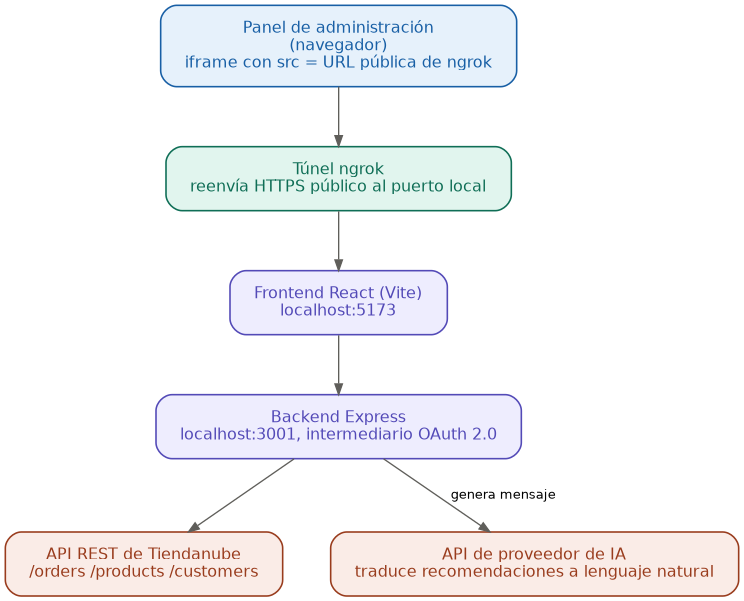
\includegraphics[width=\textwidth]{./images/diagrama_arquitectura_red.png}
    \caption{Arquitectura de red del prototipo en el entorno de desarrollo.}
    \label{fig:arquitectura-red}
\smallskip
\noindent\textit{Fuente: elaboración propia.}
\end{figure}

El flujo completo de comunicación, en el entorno de desarrollo, puede describirse en los siguientes pasos:

\begin{enumerate}
    \item Dentro del panel de administración de la tienda (servido por Tiendanube), el comerciante accede a la sección correspondiente a la aplicación, que Tiendanube renderiza como un \emph{iframe} cuyo origen (\texttt{src}) es la URL pública HTTPS provista por ngrok.

    \item ngrok reenvía el tráfico recibido en esa URL pública hacia el servidor de desarrollo de Vite, expuesto localmente en el puerto 5173, que sirve el frontend de React.

    \item Una vez cargado dentro del \emph{iframe}, el frontend inicializa el SDK Nexo, que establece comunicación con la ventana del panel de administración (la ventana padre) para obtener el contexto de la tienda y habilitar la sesión de la aplicación para ese comercio en particular.

    \item El frontend, aunque accedido a través de la URL pública de ngrok, se ejecuta en el navegador de la misma máquina donde corre el entorno de desarrollo. Por lo tanto, sus llamadas a la API propia de la aplicación se realizan directamente contra el backend en \texttt{localhost:3001}, sin necesidad de atravesar el túnel de ngrok.

    \item El backend, sobre la base del token obtenido mediante el flujo OAuth 2.0 descripto en el CU-01 (Sección~\ref{sec:cu-01}), consume los recursos correspondientes de la API REST de Tiendanube (\texttt{/orders}, \texttt{/products}, \texttt{/customers}, entre otros, detallados en la Sección~\ref{sec:recursos-campos}) \parencite{TiendanubeAPI2024}, y devuelve al frontend los datos ya procesados.

    \item El frontend renderiza la respuesta dentro del \emph{iframe}, integrada visualmente al panel de administración mediante los componentes de Nimbus.
\end{enumerate}

Esta topología de red es propia del entorno de desarrollo y depende de un túnel de terceros (ngrok) en lugar de una infraestructura de \emph{hosting} propia. Tal como se detalla en la Sección~\ref{sec:tunel-ngrok}, esta elección fue evaluada frente a una plataforma de despliegue (Vercel) y resulta adecuada para el desarrollo. El prototipo desplegado reemplaza el túnel por el servicio de nginx en Railway, que sirve la aplicación desde una URL pública y estable (Sección~\ref{sec:infraestructura} y Figura~\ref{fig:despliegue}); lo que queda fuera del alcance es el despliegue a escala industrial, no el del prototipo.

En la tienda de desarrollo de Tiendanube se verificó que la aplicación carga embebida dentro del \emph{iframe} del panel de administración, con el intercambio (\emph{handshake}) de Nexo funcionando de forma correcta entre el \emph{iframe} y la ventana padre. Esta verificación no constituye una prueba de punta a punta de la integración: la sincronización, la generación de recomendaciones y los \emph{webhooks} se probaron de punta a punta con una tienda WooCommerce (Sección~\ref{sec:conclusiones-especificos}).

\subsection{Diagrama de componentes}
\label{sec:diagrama-componentes}

Mientras que la Figura~\ref{fig:arquitectura-red} describe la topología de red del prototipo, la Figura~\ref{fig:comp-diagram} desciende un nivel de detalle y presenta los componentes internos del frontend y de los dos procesos del backend, la API y el worker, junto con los servicios externos con los que interactúan.

\begin{figure}[!htbp]
    \centering
    \begin{tikzpicture}[
    comp/.style={draw, fill=white, rounded corners=1pt, align=center, font=\footnotesize,
        text width=4.0cm, minimum height=1cm, execute at begin node={\hyphenpenalty=10000}},
    ext/.style={draw, fill=gray!18, rounded corners=1pt, align=center, font=\footnotesize,
        text width=3.0cm, minimum height=1cm, execute at begin node={\hyphenpenalty=10000}},
    capa/.style={draw, fill=gray!6, rounded corners=2pt},
    tit/.style={font=\scriptsize\bfseries, anchor=north west, inner sep=3pt},
    titd/.style={tit, anchor=north east},
    flecha/.style={-{Stealth[length=5pt]}, thin},
    doble/.style={{Stealth[length=5pt]}-{Stealth[length=5pt]}, thin},
    etiq/.style={font=\scriptsize, fill=gray!6, inner sep=1pt, align=center}]

  % Capas
  \draw[capa] (0.3,0) rectangle (11.25,-2.1);
  \node[tit] at (0.3,0) {Frontend (React y Nimbus)};
  \draw[capa] (0.3,-2.8) rectangle (11.25,-7.0);
  \node[titd] at (11.25,-2.8) {Backend: API (Node.js y Express)};
  \draw[capa] (0.3,-7.7) rectangle (11.25,-13.9);
  \node[titd] at (11.25,-7.7) {Backend: worker (Node.js y cola de trabajos pg-boss)};
  \draw[capa] (12.35,-2.8) rectangle (15.9,-13.9);
  \node[tit] at (12.35,-2.8) {Servicios externos};

  % Frontend
  \node[comp] (panel) at (2.75,-1.2) {Panel de recomendaciones};
  \node[comp] (sesion) at (8.8,-1.2) {Cliente Nexo (Tiendanube) o complemento de WordPress (WooCommerce)};

  % API
  \node[comp] (apiapp) at (2.75,-3.9) {API de la aplicación (recomendaciones y \emph{feedback})};
  \node[comp] (webhooks) at (8.8,-3.9) {Manejador de \emph{webhooks} (privacidad y eventos de la tienda)};
  \node[comp] (conexion) at (8.8,-5.9) {Conexión de tiendas (OAuth de Tiendanube y claves de WooCommerce)};

  % Worker
  \node[comp] (cola) at (2.75,-8.8) {Cola de trabajos y trabajos programados};
  \node[comp] (ingesta) at (8.8,-8.8) {Módulo de ingesta (ETL) con adaptadores de plataforma};
  \node[comp] (motor) at (2.75,-10.6) {Motor de reglas por rubro, con la capa predictiva};
  \node[comp] (mensajes) at (8.8,-10.6) {Generador de mensajes};
  \node[comp] (scoring) at (2.75,-12.4) {Módulo de \emph{scoring} dinámico (bandit e impacto)};
  \node[comp] (cambio) at (8.8,-12.4) {Consultor de tipo de cambio};

  % Base de datos
  \node[draw, cylinder, shape border rotate=90, aspect=0.18, fill=white, minimum height=1.2cm,
        minimum width=3.6cm, font=\footnotesize, align=center] (bd) at (5.78,-15.2) {PostgreSQL (Prisma)};

  % Servicios externos
  \node[ext, minimum height=6.1cm] (plataformas) at (14.15,-6.35) {Plataformas de comercio electrónico:\\[4pt] API REST de Tiendanube\\[4pt] API REST de WooCommerce de cada tienda};
  \node[ext] (ia) at (14.15,-10.6) {API del proveedor de IA (Gemini)};
  \node[ext] (dolar) at (14.15,-12.4) {API pública de tipo de cambio (DolarApi)};

  % Relaciones
  \draw[flecha, dashed] (sesion) -- node[etiq, above=3pt]{sesión} (panel);
  \draw[flecha] (panel) -- node[etiq, right=2pt]{HTTP/JSON} (apiapp);
  \draw[flecha] (plataformas.west |- webhooks) -- node[etiq, above=2pt]{\emph{webhooks}} (webhooks);
  \draw[doble] (conexion) -- node[etiq, above=2pt]{OAuth 2.0} (plataformas.west |- conexion);
  \draw[flecha] (apiapp |- 0,-7.0) -- node[etiq, right=2pt]{encolan trabajos} (cola);
  \draw[flecha] (cola) -- node[etiq, above=2pt]{ejecuta} (ingesta);
  \draw[flecha] (cola) -- node[etiq, right=2pt]{ejecuta} (motor);
  \draw[flecha] (ingesta) -- node[etiq, above=2pt]{HTTP GET} (plataformas.west |- ingesta);
  \draw[flecha] (motor) -- node[etiq, above=2pt]{delega la\\ redacción} (mensajes);
  \draw[flecha] (mensajes) -- node[etiq, above=2pt]{HTTP POST} (ia);
  \draw[flecha] (cambio) -- node[etiq, above=2pt]{HTTP GET} (dolar);
  \draw[doble] (motor) -- node[etiq, right=2pt]{prioriza} (scoring);
  \draw[flecha, dashed] (5.78,-13.9) -- node[font=\scriptsize, right=2pt]{lee y escribe} (bd.north);
  \draw[flecha, dashed] (0.3,-4.9) -- (0.05,-4.9) |- node[font=\scriptsize, pos=0.75, above=1pt]{lee y escribe} (bd.west);
\end{tikzpicture}

    \caption{Diagrama de componentes del prototipo.}
    \label{fig:comp-diagram}
\smallskip
\noindent\textit{Fuente: elaboración propia.}
\end{figure}

El frontend, embebido en el \emph{iframe} del panel de administración de Tiendanube o de WordPress, se compone del panel de recomendaciones, que consume la API propia de la aplicación mediante HTTP, y del componente que establece la sesión: el cliente Nexo, que resuelve el \emph{handshake} descripto en la Sección~\ref{sec:arquitectura-red}, o el complemento de WordPress, que entrega un token firmado (Sección~\ref{sec:autenticacion}). El backend se divide en dos procesos. La API atiende al frontend y a las plataformas: la API de la aplicación expone las recomendaciones y registra el \emph{feedback} del comerciante; la conexión de tiendas implementa la autenticación OAuth de Tiendanube descripta en el CU-01 (Sección~\ref{sec:cu-01}) y la conexión de WooCommerce del CU-09 (Sección~\ref{sec:cu-09}); y el manejador de \emph{webhooks} recibe las solicitudes de privacidad del CU-07 (Sección~\ref{sec:cu-07}) y los eventos de la tienda. El worker ejecuta los trabajos que encola la API y los trabajos programados (Sección~\ref{sec:infraestructura}): el módulo de ingesta (ETL) implementa el CU-02 (Sección~\ref{sec:cu-02}) mediante los adaptadores de cada plataforma (Sección~\ref{sec:multiplataforma}); el consultor de tipo de cambio corresponde al CU-08 (Sección~\ref{sec:cu-08}); y el motor de reglas por rubro, junto con el módulo de scoring dinámico, implementa el CU-03 (Sección~\ref{sec:cu-03}). El motor delega en un generador de mensajes que invoca la API externa del proveedor de IA para traducir cada recomendación a lenguaje natural (RF-19). Los dos procesos persisten y consultan su información en la base de datos PostgreSQL presentada en las Figuras~\ref{fig:der-catalogo} a~\ref{fig:der-motor}, que aloja también la cola de trabajos, y acceden a los datos externos exclusivamente a través de las API de las plataformas, del proveedor de IA y de tipo de cambio.

\subsection{Entorno de desarrollo}
\label{sec:entorno-desarrollo}

Levantar el entorno de desarrollo completo requiere ejecutar tres procesos en simultáneo: el backend (\texttt{cd backend \&\& npm run dev}, puerto 3001), el frontend (\texttt{cd frontend \&\& npm run dev}, puerto 5173) y el túnel de ngrok (\texttt{ngrok http 5173}). Esta separación en tres procesos independientes refleja directamente la arquitectura de red descripta en la Sección~\ref{sec:arquitectura-red}: cada uno de ellos corresponde a un componente distinto del flujo de comunicación (servidor de API, servidor de la interfaz y túnel público).

La configuración de cada capa se administra mediante variables de entorno independientes en cada carpeta del monorepo. El backend concentra las credenciales sensibles de la aplicación (\texttt{Client ID} y \texttt{Client Secret} de Tiendanube), mientras que el frontend recibe únicamente el \texttt{Client ID}, dato público necesario para inicializar el SDK Nexo del lado del navegador. Esta separación no es incidental: mantiene el \texttt{Client Secret} fuera del código que se ejecuta en el navegador del usuario, en línea con el rol del backend como intermediario autenticado descripto en la Sección~\ref{sec:backend-node-express}. Cabe señalar, además, que Vite solo lee las variables de entorno del frontend al iniciar el proceso, por lo que una modificación en su archivo de configuración requiere reiniciar el servidor de desarrollo correspondiente para que los nuevos valores se apliquen.

\subsection{Infraestructura y despliegue}
\label{sec:infraestructura}

El prototipo está diseñado para ejecutarse como tres servicios independientes: la API (\texttt{backend/src/index.js}), el worker de procesamiento asíncrono (\texttt{backend/src/worker.js}) y el frontend estático servido con nginx. La separación entre API y worker responde a la arquitectura de cola de trabajos basada en pg-boss: los procesos de alta latencia ---sincronización de datos, ejecución del motor de análisis, pronóstico de demanda, segmentación de clientes y consulta diaria del tipo de cambio--- corren en el worker como trabajos en segundo plano, mientras que la API permanece sin estado y disponible para responder las consultas del frontend. La cola está alojada en la misma base de datos PostgreSQL de Neon, lo que elimina la necesidad de una infraestructura de mensajería adicional.

El repositorio incluye un \texttt{docker-compose.yml} que levanta el entorno de desarrollo completo ---backend, worker y frontend--- mediante un único comando, con recarga en caliente. Un perfil adicional (\texttt{local-db}) incorpora una instancia de PostgreSQL local como alternativa a Neon, de modo que cualquier persona pueda clonar el repositorio y ejecutar el sistema completo sin depender de servicios externos; esto es un requisito de reproducibilidad del prototipo.

El prototipo se despliega en Railway como tres servicios construidos a partir del mismo repositorio, cada uno con su propio archivo de configuración \texttt{railway.json}. La API aplica al arrancar las migraciones pendientes de la base de datos (\texttt{prisma migrate deploy}) y expone un punto de verificación de estado (\texttt{/api/health}) que Railway consulta antes de considerar activo el servicio. El worker ejecuta la cola de trabajos y los trabajos programados sin exponer ningún puerto. El frontend es una imagen de nginx que sirve los archivos estáticos generados por Vite. Los tres servicios se reinician automáticamente ante una falla. La Figura~\ref{fig:despliegue} resume el despliegue. A diferencia de la Figura~\ref{fig:arquitectura-red}, que corresponde al entorno de desarrollo, el navegador del comerciante carga la aplicación desde el servicio de nginx. La API cuenta, además, con un dominio público propio, al que Tiendanube redirige el flujo de OAuth y al que las plataformas envían sus \emph{webhooks}.

\begin{figure}[!htbp]
    \centering
    \begin{tikzpicture}[
    serv/.style={draw, fill=white, rounded corners=1pt, align=left, font=\footnotesize,
        text width=4.8cm, inner sep=4pt, execute at begin node={\hyphenpenalty=10000}},
    ext/.style={draw, fill=gray!18, rounded corners=1pt, align=center, font=\footnotesize,
        text width=3.6cm, minimum height=1cm, execute at begin node={\hyphenpenalty=10000}},
    capa/.style={draw, fill=gray!6, rounded corners=2pt},
    tit/.style={font=\scriptsize\bfseries, anchor=north west, inner sep=3pt},
    flecha/.style={-{Stealth[length=5pt]}, thin},
    doble/.style={{Stealth[length=5pt]}-{Stealth[length=5pt]}, thin},
    etiq/.style={font=\scriptsize, fill=white, inner sep=1pt, align=center}]

  % Navegador del comerciante
  \draw[capa] (0,0) rectangle (3.4,-3.4);
  \node[tit] at (0,0) {Navegador del comerciante};
  \node[draw, fill=white, rounded corners=1pt, font=\footnotesize, align=center, text width=2.8cm,
        execute at begin node={\hyphenpenalty=10000}] (iframe) at (1.7,-2.0)
      {Panel de Tiendanube o de WordPress, con la aplicación en un \emph{iframe}};

  % Railway
  \draw[capa] (4.1,0) rectangle (10.7,-9.5);
  \node[tit] at (4.1,0) {Railway (tres servicios del mismo repositorio)};
  \node[serv] (front) at (7.4,-1.95) {\textbf{frontend}: nginx\\
      Sirve los archivos estáticos generados por Vite.\\
      CSP \texttt{frame-ancestors}: Tiendanube y WordPress.\\
      Reenvía \texttt{/api/} a la API.};
  \node[serv] (api) at (7.4,-4.95) {\textbf{api}: Express y Prisma\\
      Aplica las migraciones al arrancar.\\
      Verificación de estado en \texttt{/api/health}.\\
      Dominio público propio para OAuth y \emph{webhooks}.};
  \node[serv] (worker) at (7.4,-7.95) {\textbf{worker}: pg-boss\\
      Sincronización cada 6 horas, tipo de cambio diario y evaluación de impacto diaria.\\
      Sin puertos expuestos.};

  % Neon
  \draw[capa] (4.1,-10.2) rectangle (10.7,-12.6);
  \node[tit] at (4.1,-10.2) {Neon (PostgreSQL)};
  \node[draw, fill=white, rounded corners=1pt, font=\footnotesize, align=center, text width=4.8cm,
        execute at begin node={\hyphenpenalty=10000}] (neon) at (7.4,-11.55)
      {Rama \texttt{main}: producción, con la cola de pg-boss\\ (separada de las ramas de desarrollo)};

  % Servicios externos
  \draw[capa] (11.4,0) rectangle (15.9,-9.5);
  \node[tit] at (11.4,0) {Servicios externos};
  \node[ext, minimum height=3.4cm] (plataformas) at (13.65,-4.25) {Plataformas:\\[3pt] API REST de Tiendanube\\[3pt] tiendas WooCommerce de los comerciantes};
  \node[ext] (ia) at (13.65,-7.4) {API de Gemini};
  \node[ext] (dolar) at (13.65,-8.8) {DolarApi};

  % Conexiones
  \draw[flecha] (iframe.east |- front) -- node[etiq, above=2pt]{HTTPS} (front);
  \draw[flecha] (front) -- node[etiq, right=2pt]{\texttt{/api/}} (api);
  \draw[doble] (api.east |- 0,-4.95) -- node[etiq, above=2pt, align=center]{OAuth y\\ \emph{webhooks}} (plataformas.west |- 0,-4.95);
  \draw[flecha] (worker.north east) -- node[etiq, sloped, above=1pt]{sincronización} (plataformas.south west);
  \draw[flecha] (worker.east |- ia) -- node[etiq, above=2pt]{redacción} (ia);
  \draw[flecha] (worker.east |- dolar) -- node[etiq, above=2pt]{cotización} (dolar);
  \draw[flecha] (api.west) -- ++(-0.45,0) |- node[etiq, pos=0.25, left=2pt, align=right]{\emph{pooler} de\\ conexiones} ([yshift=0.2cm]neon.west);
  \draw[flecha] (worker) -- node[etiq, right=2pt]{conexión directa} (neon);
\end{tikzpicture}

    \caption{Diagrama de despliegue del prototipo en Railway y Neon.}
    \label{fig:despliegue}

    \smallskip
    \noindent\textit{Fuente: elaboración propia sobre la base de la configuración de despliegue del prototipo.}
\end{figure}

nginx cumple, además, una función de seguridad y otra de enrutamiento, ambas configuradas mediante variables de entorno al iniciar el contenedor. \texttt{FRAME\_ANCESTORS} define, en el encabezado \texttt{Content-Security-Policy}, los únicos orígenes autorizados a embeber la aplicación en un \emph{iframe}: los paneles de administración de Tiendanube y los orígenes de WordPress configurados para WooCommerce. \texttt{API\_UPSTREAM} indica el servicio de la API al que nginx reenvía las solicitudes dirigidas a \texttt{/api/}, de modo que el navegador se comunica con un único origen.

La base de datos se aloja en Neon, en su rama principal (\texttt{main}), que funciona como rama de producción, separada de las ramas de desarrollo. La API se conecta a ella a través del \emph{pooler} de conexiones de Neon, mientras que el worker usa una conexión directa, que requiere la cola de pg-boss. Las credenciales y claves de cada servicio se cargan como variables de entorno en Railway, fuera del repositorio. La misma imagen de Docker puede trasladarse a AWS sin cambios, migración que queda como trabajo futuro.

Las Tablas~\ref{tab:comparativo_hosting}, \ref{tab:comparativo_bd_nube} y~\ref{tab:comparativo_cola} resumen la comparación con la que se eligieron el proveedor de despliegue, el servicio de base de datos y el mecanismo de cola de trabajos. Como en el resto del stack, la comparación se apoya en las características documentadas de cada opción y en su adecuación al alcance de un prototipo. Railway se eligió porque despliega los tres servicios desde el mismo repositorio y ejecuta el worker como un proceso de larga duración, sin adaptarlo a un modelo \emph{serverless}; AWS queda como camino de migración, ya que admite las mismas imágenes de Docker. Neon se eligió por las ramas de la base de datos, que permiten que cada integrante trabaje sobre una copia aislada (Sección~\ref{sec:eval-generacion}), por su \emph{pooler} de conexiones y por su plan gratuito; sus limitaciones son el arranque en frío después de un período sin uso, la cuota de cómputo del plan y la dependencia de un tercero. pg-boss se eligió porque aloja la cola en la misma base de datos PostgreSQL y evita sumar un servicio de mensajería.

\begin{table}[h]
\centering
\caption{Comparación de proveedores para desplegar el prototipo}
\label{tab:comparativo_hosting}
\renewcommand{\arraystretch}{1.3}
\begin{tabular}{|m{2.3cm}|m{4.4cm}|m{4.4cm}|m{3.4cm}|}
\hline
\textbf{Opción} & \textbf{Ventajas} & \textbf{Consideraciones} & \textbf{Decisión} \\
\hline
Railway & Despliega la API, el worker y el frontend como tres servicios del mismo repositorio, con imágenes de Docker y un archivo de configuración por servicio; ejecuta procesos de larga duración; verificación de estado y reinicio automático ante fallas & Dependencia de un proveedor externo; los recursos están limitados por el plan contratado & \textbf{Elegido} para el despliegue del prototipo \\
\hline
Render & Servicios web y procesos en segundo plano a partir de imágenes de Docker & Capacidades equivalentes a las de Railway para el alcance del prototipo & Alternativa válida, sin una ventaja decisiva frente a Railway \\
\hline
AWS (ECS Fargate o App Runner) & Mayor control y capacidad de escalar; admite las mismas imágenes de Docker sin cambios & Mayor complejidad de configuración: clúster, definiciones de tareas, balanceador de carga y gestión de secretos & Descartado para el prototipo; queda como camino de migración \\
\hline
\end{tabular}
\end{table}

\begin{table}[h]
\centering
\caption{Comparación de servicios para alojar la base de datos PostgreSQL}
\label{tab:comparativo_bd_nube}
\renewcommand{\arraystretch}{1.3}
\begin{tabular}{|m{2.3cm}|m{4.4cm}|m{4.4cm}|m{3.4cm}|}
\hline
\textbf{Opción} & \textbf{Ventajas} & \textbf{Consideraciones} & \textbf{Decisión} \\
\hline
Neon & PostgreSQL \emph{serverless}; \emph{pooler} de conexiones; ramas de la base por desarrollador, creadas por copia en escritura \parencite{NeonBranching2026}; plan gratuito & Arranque en frío después de un período sin uso; cuota de cómputo del plan; dependencia de un tercero & \textbf{Elegido} \\
\hline
PostgreSQL de Railway & Misma plataforma que los servicios desplegados & No ofrece el flujo de trabajo con una rama de la base por desarrollador que usa el equipo & Descartado: el flujo de ramas pesó más que unificar el proveedor \\
\hline
Amazon RDS & Mayor control sobre la instancia y la configuración & Mayor trabajo de configuración y administración para un prototipo & Descartado para el prototipo; opción de migración si el volumen de conexiones supera el plan de Neon \\
\hline
Instalación local (Docker) & Sin dependencia de servicios externos; reproducible & No es accesible desde los servicios desplegados ni se comparte entre los integrantes & Alternativa para ejecutar el sistema localmente (Sección~\ref{sec:infraestructura}) \\
\hline
\end{tabular}
\end{table}

\begin{table}[h]
\centering
\caption{Comparación de mecanismos para la cola de trabajos}
\label{tab:comparativo_cola}
\renewcommand{\arraystretch}{1.3}
\begin{tabular}{|m{2.3cm}|m{4.4cm}|m{4.4cm}|m{3.4cm}|}
\hline
\textbf{Opción} & \textbf{Ventajas} & \textbf{Consideraciones} & \textbf{Decisión} \\
\hline
pg-boss & Cola persistida en la misma base PostgreSQL, sin infraestructura de mensajería adicional; trabajos programados y reintentos & Requiere una conexión directa a la base, no a través del \emph{pooler}; la consulta periódica de la cola consume cómputo de la base & \textbf{Elegido} \\
\hline
BullMQ con Redis & Biblioteca de colas madura y de alto rendimiento & Requiere desplegar y mantener un servicio de Redis adicional & Descartado: suma infraestructura sin un beneficio para el volumen del prototipo \\
\hline
Tareas en el mismo proceso de la API & Sin dependencias ni procesos adicionales & Los procesos de alta latencia competirían con las consultas del panel; los trabajos en curso se pierden si el proceso se reinicia; impide mantener la API sin estado & Descartado \\
\hline
\end{tabular}
\end{table}

\subsection{Seguridad}
\label{sec:seguridad}

Esta subsección consolida los controles de seguridad implementados en el prototipo. El análisis de amenazas que guió las decisiones aplica el modelo STRIDE ---suplantación de identidad (\emph{Spoofing}), manipulación de datos (\emph{Tampering}), repudio (\emph{Repudiation}), divulgación de información (\emph{Information Disclosure}), denegación de servicio (\emph{Denial of Service}) e incremento de privilegios (\emph{Elevation of Privilege})--- sobre los componentes del sistema descripto en la Figura~\ref{fig:comp-diagram}.

\subsubsection{Autenticación y aislamiento entre tiendas}
\label{sec:autenticacion}

El backend no mantiene estado de sesión en el servidor: cada solicitud se autentifica de forma independiente a partir del token enviado en el encabezado \texttt{Authorization}. Para tiendas de Tiendanube, el frontend obtiene un JWT de sesión mediante el SDK Nexo; el backend lo verifica como JWT HS256 firmado con \texttt{TIENDANUBE\_CLIENT\_SECRET} mediante \texttt{timingSafeEqual} y comprueba su expiración. Para tiendas de WooCommerce, el complemento de WordPress envía un token de dos segmentos firmado con HMAC; el registro de la plataforma lo valida y resuelve la tienda correspondiente. En ambos casos, el middleware establece el objeto \texttt{req.store} y ninguna ruta acepta un \texttt{store\_id} externo: toda consulta filtra por la tienda de la sesión verificada, lo que impide que una tienda acceda a los datos de otra.

\subsubsection{Cifrado de credenciales}
\label{sec:cifrado-credenciales}

Los datos sensibles almacenados en la base de datos se cifran con AES-256-GCM: el token de acceso OAuth de Tiendanube y las credenciales del plugin de WooCommerce (\texttt{consumer\_key}, \texttt{consumer\_secret} y \texttt{plugin\_secret}). El módulo \texttt{backend/src/security/crypto.js} genera un vector de inicialización aleatorio por operación y produce una cadena con el formato \texttt{1:<iv\_hex>:<tag\_hex>:<ciphertext\_hex>}, que incluye el \emph{tag} de autenticación del modo GCM para detectar cualquier alteración del texto cifrado. La clave de 32 bytes se lee de la variable de entorno \texttt{TOKEN\_ENCRYPTION\_KEY}; si no está configurada o no tiene la longitud correcta, el proceso se niega a arrancar.

Las credenciales que se almacenaban en texto plano antes de incorporar el cifrado se migran con el script \texttt{migrate-encrypt-tokens.js}. El script verifica primero que la clave cifre y descifre correctamente, cifra cada token pendiente y omite los que ya están cifrados, por lo que puede ejecutarse más de una vez sin efectos adicionales. En producción, la clave se carga como variable de entorno de los servicios en Railway (Sección~\ref{sec:infraestructura}); su pérdida vuelve irrecuperables los tokens cifrados y obliga a reconectar las tiendas.

\subsubsection{Verificación de webhooks}
\label{sec:webhooks-hmac}

Los \emph{webhooks} de Tiendanube se verifican con HMAC-SHA256: el middleware \texttt{requireWebhookHmac} captura el cuerpo crudo de la solicitud antes del parseo JSON, calcula el HMAC con \texttt{TIENDANUBE\_CLIENT\_SECRET} y compara el resultado con el encabezado \texttt{x-linkedstore-hmac-sha256} mediante \texttt{timingSafeEqual}. Una firma inválida devuelve~401 y registra el intento en el log. Este control protege los tres \emph{webhooks} de privacidad (\texttt{/api/webhooks/store-redact}, \texttt{customers-redact} y \texttt{customers-data-request}) contra solicitudes no autorizadas que podrían desencadenar borrados de datos.

\subsubsection{Privacidad y Ley 25.326}
\label{sec:privacidad-ley}

Los tres \emph{webhooks} de privacidad implementan los derechos de los titulares de datos personales previstos en la Ley~25.326 de Protección de los Datos Personales de la República Argentina \parencite{Ley25326} y en el Reglamento General de Protección de Datos (RGPD) de la Unión Europea:

\begin{itemize}
    \item \textbf{Supresión de la tienda} (\texttt{store-redact}): elimina en una transacción todos los datos de la tienda ---categorías, productos, variantes, fotos de stock, clientes, pedidos, recomendaciones, pronósticos, segmentación, brazos del bandit y configuraciones--- incluyendo la propia entrada de la tienda.
    \item \textbf{Supresión del cliente} (\texttt{customers-redact}): anonimiza al cliente (nombre, correo electrónico, DNI, teléfono, dirección y notas) y elimina su segmentación, conservando sus pedidos sin datos personales porque son necesarios para las métricas del motor de análisis.
    \item \textbf{Acceso} (\texttt{customers-data-request}): reúne todos los datos del cliente que el sistema almacena para su entrega al titular.
\end{itemize}

El procesamiento de cada solicitud es idempotente: recibir la misma solicitud dos veces no duplica ni revierte el borrado. La tabla \texttt{PRIVACY\_REQUESTS} actúa como registro de auditoría con el tipo de solicitud, los identificadores de la tienda y del cliente, y las marcas temporales de recepción y procesamiento. La finalidad del tratamiento de datos se limita a la generación de recomendaciones comerciales; el prototipo no cede datos a terceros y puede suprimir o anonimizar los datos de un titular ante una solicitud fundada.

\subsubsection{Anonimización de datos enviados al proveedor de IA}
\label{sec:anonimizacion-llm}

En desarrollo, el prototipo utiliza la capa gratuita de la API de Gemini, cuyos términos de servicio permiten que el contenido enviado se use para mejorar los productos de Google; en producción utiliza el plan pago, cuyo contenido no se usa para entrenar modelos \parencite{GoogleGeminiTerms2026}. El módulo \texttt{backend/src/security/llmSanitizer.js} construye el contenido del \emph{prompt} a partir de una lista blanca de campos permitidos: tipo de recomendación, rubro, métricas numéricas y nombres de productos y variantes. Los nombres de clientes se reemplazan por el marcador \texttt{\{\{cliente\}\}} antes de la llamada a la API; el backend restaura el nombre real en el texto devuelto por Gemini antes de persistirlo. El módulo también elimina correos electrónicos, DNIs (secuencias de siete u ocho dígitos) y enlaces de cualquier texto de la tienda.

\subsubsection{Mitigación de inyección de prompt}
\label{sec:prompt-injection}

Los nombres de productos, variantes y clientes que provienen de la tienda son datos no confiables que podrían contener instrucciones diseñadas para manipular el comportamiento del modelo de lenguaje. El prototipo aplica tres controles complementarios:

\begin{enumerate}
    \item \textbf{Separación de instrucciones y datos:} el \emph{system prompt} contiene exclusivamente las instrucciones para el modelo; la información de la recomendación viaja en el contenido del usuario delimitada por las etiquetas \texttt{<datos\_tienda>} y \texttt{</datos\_tienda>}. El \emph{system prompt} instruye explícitamente al modelo a tratar todo el contenido del bloque solo como datos y a ignorar cualquier pedido o enlace que aparezca en él.
    \item \textbf{Sanitización de los textos de la tienda:} la función \texttt{sanitizeStoreText} normaliza cada texto antes de incluirlo en el bloque: elimina caracteres de control e invisibles (categorías Unicode $\{Cc\}$ y $\{Cf\}$, separadores de línea y párrafo), reemplaza los delimitadores del bloque (\texttt{<} y \texttt{>}) y los marcadores del sanitizador (\texttt{\{\{} y \texttt{\}\}}) para que ningún texto de la tienda pueda imitarlos, y aplica un límite de 120 caracteres por campo.
    \item \textbf{Validación de la respuesta:} la función \texttt{validateOutput} verifica que el texto generado cumpla con criterios predefinidos: largo máximo por campo (\texttt{message}: 300 caracteres; \texttt{detail\_reason}: 1\,200), ausencia de URLs o dominios, y mención del objetivo de la recomendación. Una respuesta que no supera la validación se descarta y el sistema usa la plantilla de respaldo sin exponer el error al usuario.
\end{enumerate}

\subsubsection{Endurecimiento general}
\label{sec:endurecimiento}

El backend aplica encabezados de seguridad mediante \texttt{helmet}, con una política de \texttt{Content-Security-Policy} configurada para que la aplicación funcione dentro de los \emph{iframes} de Tiendanube y WordPress. El acceso desde otros orígenes queda restringido mediante CORS al origen del frontend, y un limitador de tasa (\texttt{express-rate-limit}) aplica umbrales más estrictos en los \emph{endpoints} de escritura y en el \emph{endpoint} de generación manual. La validación de entradas en todos los \emph{endpoints} se implementa con Zod: una solicitud con cuerpo inválido devuelve~400 con un mensaje descriptivo. Los registros de sistema omiten automáticamente los campos sensibles. Como limitación del prototipo, la gestión de secretos se realiza mediante variables de entorno sin un sistema de rotación automatizado; la incorporación de un servicio dedicado queda como trabajo futuro (Sección~\ref{sec:conclusiones-futuro}).

\section{Arquitectura del motor de inteligencia artificial}
\label{sec:motor-ia}

El Marco Teórico presentó el enfoque híbrido en tres capas sobre el que se organiza el motor de recomendaciones (Sección~\ref{sec:sistemas-recomendacion}): una capa predictiva, una capa de reglas de negocio por rubro y una capa de aprendizaje por refuerzo para la priorización, a las que se suma un modelo de lenguaje que solo redacta. Esta sección describe cómo el prototipo implementa cada capa: el flujo de datos que las conecta, los algoritmos con sus parámetros, las seis reglas con sus umbrales por rubro, el calendario de fechas clave, la regla de actualización del bandit y el criterio con el que se ordenan las recomendaciones. Cierra con la forma en que se evalúa el motor, cuyos resultados se presentan en la Sección~\ref{sec:evaluacion-modelos}.

\subsection{Flujo de datos entre las capas}
\label{sec:motor-flujo}

El motor se ejecuta en el proceso de tareas en segundo plano (\emph{worker}), separado de la API, y se encadena a la sincronización de los datos de cada tienda. La Figura~\ref{fig:motor-capas} resume el recorrido. Cada sincronización, ya sea la incremental, que se repite cada seis horas, o la que disparan los webhooks de la plataforma, deja los datos en el modelo canónico del sistema y encola el recálculo del pronóstico de demanda y de la segmentación de clientes (capa predictiva). Al terminar, se encola la ejecución del motor, que resuelve el rubro de la tienda, aplica las seis reglas sobre las predicciones (capa de reglas) y asigna a cada recomendación el puntaje de su tipo según el bandit (capa de priorización). Antes de guardarla, el modelo de lenguaje redacta su mensaje (capa de explicación). Cuando el comerciante abre el panel, la API ordena las recomendaciones activas con una muestra de Thompson Sampling del día.

\begin{figure}[!htbp]
\centering
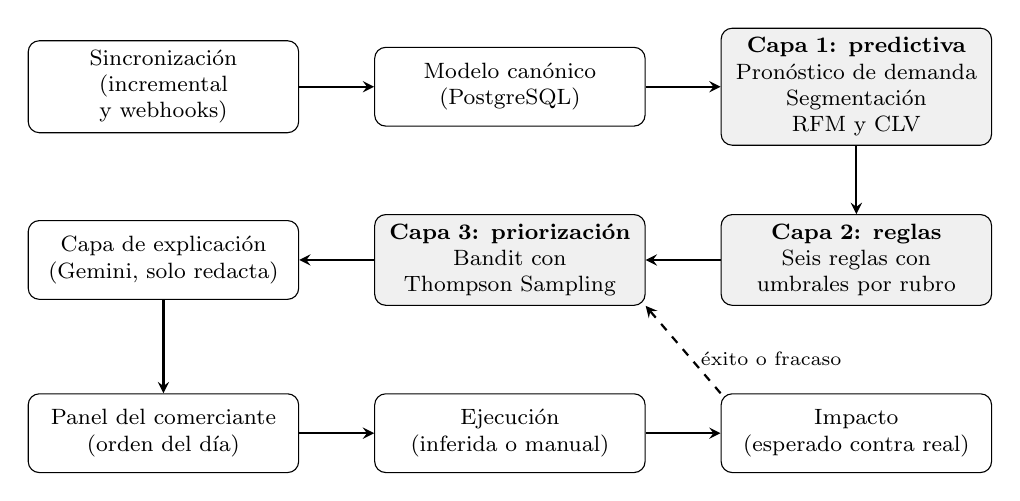
\begin{tikzpicture}[
    caja/.style={draw, rounded corners, align=center, font=\footnotesize, minimum height=1cm, text width=3.2cm},
    capa/.style={caja, fill=gray!12},
    flecha/.style={-stealth, thick}]
  \node[caja] (sync) at (0,0) {Sincronización\\(incremental y webhooks)};
  \node[caja] (canon) at (4.4,0) {Modelo canónico\\(PostgreSQL)};
  \node[capa] (pred) at (8.8,0) {\textbf{Capa 1: predictiva}\\Pronóstico de demanda\\Segmentación RFM y CLV};
  \node[capa] (reglas) at (8.8,-2.2) {\textbf{Capa 2: reglas}\\Seis reglas con\\umbrales por rubro};
  \node[capa] (bandit) at (4.4,-2.2) {\textbf{Capa 3: priorización}\\Bandit con\\Thompson Sampling};
  \node[caja] (llm) at (0,-2.2) {Capa de explicación\\(Gemini, solo redacta)};
  \node[caja] (panel) at (0,-4.4) {Panel del comerciante\\(orden del día)};
  \node[caja] (ejec) at (4.4,-4.4) {Ejecución\\(inferida o manual)};
  \node[caja] (impacto) at (8.8,-4.4) {Impacto\\(esperado contra real)};
  \draw[flecha] (sync) -- (canon);
  \draw[flecha] (canon) -- (pred);
  \draw[flecha] (pred) -- (reglas);
  \draw[flecha] (reglas) -- (bandit);
  \draw[flecha] (bandit) -- (llm);
  \draw[flecha] (llm) -- (panel);
  \draw[flecha] (panel) -- (ejec);
  \draw[flecha] (ejec) -- (impacto);
  \draw[flecha, dashed] (impacto.north west) -- node[font=\scriptsize, right, pos=0.4] {éxito o fracaso} (bandit.south east);
\end{tikzpicture}
\caption{Capas del motor de recomendaciones y flujo de datos entre ellas.}
\label{fig:motor-capas}

\smallskip
\noindent\textit{Fuente: elaboración propia.}
\end{figure}

El ciclo se cierra con dos tareas adicionales. Después de cada sincronización incremental, la inferencia de ejecuciones compara las fotos de stock y precio de las variantes con lo que proponía cada recomendación activa. Una vez por día, a las 5 de la mañana (hora de Argentina), la evaluación de impacto compara el resultado real de las recomendaciones cuya ventana terminó con el esperado que se fijó al generarlas, registra cada resultado como éxito o fracaso en el bandit y recalcula las distribuciones previas de cada rubro.

\subsection{Capa predictiva}
\label{sec:motor-predictiva}

La capa predictiva produce dos insumos para las reglas: el pronóstico diario de unidades de cada variante y la segmentación de los clientes de la tienda.

\paragraph{Pronóstico de demanda.} Para cada variante se construye la serie de unidades vendidas por día en órdenes pagadas, con hasta 180 días de historia y los días cortados en hora de Argentina. La serie comienza en la primera venta, porque los ceros previos a la publicación del producto no son demanda. Sobre esa historia se elige el modelo según tres casos:

\begin{itemize}
    \item con menos de 14 días de historia, suavizado exponencial simple;
    \item si más del 60\% de los días no registra ventas (demanda intermitente), promedio móvil de los últimos 28 días, marcado como pronóstico de baja confianza;
    \item en los demás casos, Holt-Winters aditivo con estacionalidad semanal ($m = 7$).
\end{itemize}

Los parámetros de suavizado se eligen por búsqueda en grilla, minimizando el error cuadrático de los pronósticos a un paso: $\alpha$ y $\gamma$ toman los valores 0,05; 0,1; 0,2; 0,3; 0,5; 0,7 y 0,9, y $\beta$, los valores 0,01; 0,05; 0,1 y 0,2. La tendencia se limita a valores bajos para que no se dispare al extrapolar dos o tres semanas. El horizonte del pronóstico es el mayor entre 14 días, el umbral de alerta de quiebre y la ventana de impacto del rubro, y la ventana completa de una fecha clave recomendada con su anticipación; en la práctica, 17 días para gastronomía e indumentaria y 21 para electrónica. Antes de pronosticar, el modelo se valida reservando los últimos 14 días de la serie: se ajusta con el resto y su WAPE se compara con el de dos referencias, un pronóstico plano igual al promedio de los últimos 28 días y uno semanal ingenuo que repite la última semana observada.

El efecto de las fechas clave se estima con la historia de cada tienda: para cada ocurrencia pasada de una fecha, se divide la venta total de la tienda en la ventana de la fecha por la venta esperada sin ella, calculada como el promedio del mismo día de la semana en los 28 días previos, excluidos los días de otras fechas clave. La estimación requiere al menos 14 días de referencia válidos y nunca baja de 1. Si no se puede estimar, se usa el factor típico del rubro (Tabla~\ref{tab:motor-fechas}).

\paragraph{Segmentación de clientes.} A partir de las órdenes pagadas se calculan la recencia, la frecuencia y el monto de cada cliente. Las tres variables se transforman en $[R,\ \log(1+F),\ \log(1+M)]$, donde el logaritmo reduce el peso de los pocos clientes que concentran muchas compras, y se normalizan a puntajes $z$. Sobre esos puntos se ejecuta k-means con inicialización k-means++ y semilla fija (42), para que el resultado sea reproducible, con $k \in \{3, 4, 5\}$; se conserva el valor de $k$ con mayor coeficiente de silueta. Cada grupo se etiqueta según su centroide:

\begin{itemize}
    \item \emph{campeones}: el de mayor puntaje $-R + F + M$;
    \item \emph{perdidos}: entre los demás, el de mayor recencia;
    \item \emph{en riesgo}: los grupos cuya recencia media supera el doble de su intervalo habitual entre compras;
    \item \emph{leales} u \emph{ocasionales}: los restantes, según su frecuencia esté en la media o por encima, o por debajo de ella.
\end{itemize}

El umbral de inactividad de la tienda es el máximo entre el piso del rubro y la mediana de días entre compras de sus clientes multiplicada por el factor del rubro (Tabla~\ref{tab:motor-umbrales}). El CLV de cada cliente se calcula como el ticket promedio por las compras anuales, con una antigüedad mínima de 30 días para no anualizar de más, y por la vida esperada en años, igual a la inversa de la tasa de abandono de la tienda con un tope de cinco años. Por último, para cada segmento se mide la tasa histórica de retorno: en cortes semanales, la proporción de clientes inactivos que volvieron a comprar dentro de la ventana de impacto del rubro. Esa tasa es el esperado contra el que se mide una recomendación de retención.

\subsection{Capa de reglas por rubro}
\label{sec:motor-reglas}

\paragraph{Resolución del rubro.} Las reglas usan los parámetros del rubro efectivo de la tienda. Si el rubro declarado es uno de los tres soportados, se usa ese. En otro caso, por ejemplo en las tiendas de Tiendanube que ingresan con tipo \emph{general}, se infiere de los nombres de las categorías y los productos mediante listas de palabras clave por rubro: la inferencia es concluyente si al menos tres nombres coinciden con alguna lista y un rubro reúne el 60\% de las coincidencias. Si no lo es, se usan parámetros genéricos, iguales a los de indumentaria, y la recomendación se marca para que la interfaz lo advierta.

\paragraph{Reglas.} El motor aplica seis reglas, resumidas en la Tabla~\ref{tab:motor-reglas}. Cada una decide si corresponde recomendar, con qué nivel de prioridad (urgente, atención u oportunidad) y con qué puntaje propio, de 0 a 100, que ordena las recomendaciones de un mismo tipo. Al generar la recomendación, la regla guarda también el resultado esperado contra el que luego se medirá su impacto. Las reglas no repiten una recomendación que ya está activa para el mismo objetivo.

\begin{table}[!htbp]
\centering
\caption{Reglas del motor: condición, prioridad, puntaje y esperado para medir el impacto}
\label{tab:motor-reglas}
\renewcommand{\arraystretch}{1.3}
\footnotesize
\setlength{\tabcolsep}{3pt}
\begin{tabular}{|>{\raggedright\arraybackslash}m{2.2cm}|>{\raggedright\arraybackslash}m{4.1cm}|>{\raggedright\arraybackslash}m{2.6cm}|>{\raggedright\arraybackslash}m{1.9cm}|>{\raggedright\arraybackslash}m{2.4cm}|}
\hline
\textbf{Regla} & \textbf{Condición y variables} & \textbf{Prioridad} & \textbf{Puntaje} & \textbf{Esperado} \\
\hline
Quiebre de stock (RF-08, HU-01) & Días hasta agotar el stock $d$, acumulando la demanda pronosticada día por día; recomienda si $d \le$ umbral de alerta. Solo variantes con gestión de stock & Urgente si $d \le$ umbral urgente; si no, atención & $100\,(1 - d/\text{alerta})$ & Unidades pronosticadas en la ventana de impacto \\
\hline
Preparación anticipada (HU-02) & Día pico entre 2 y 7 días adelante con pronóstico $\ge$ 130\% del promedio reciente y al menos 1 unidad; excluye pronósticos de baja confianza y, dentro de una fecha clave, los productos no destacados & Atención si el pico está a 3 días o menos; si no, oportunidad & Suba porcentual del pico & Unidades pronosticadas en la ventana de impacto \\
\hline
Fecha clave (HU-06) & Fecha del rubro entre 1 y 14 días adelante; promoción sobre los 5 productos con más unidades vendidas en los últimos 28 días; una recomendación por ocurrencia & Oportunidad & Suba esperada, $(\text{factor} - 1) \times 100$ & Pronóstico de los destacados en la ventana de la fecha, por el factor \\
\hline
Baja rotación (RF-09, HU-03) & Caída de las unidades vendidas en la última ventana del rubro frente a la anterior; recomienda si la caída $\ge$ umbral del rubro & Atención & Caída porcentual & Pronóstico de la ventana o, sin pronóstico, el ritmo reciente \\
\hline
Revisión de precio (RF-10, HU-05) & Días desde el último cambio de precio $\ge$ umbral del rubro; en tiendas en pesos, variación del dólar desde ese cambio & Oportunidad si el dólar subió más que el umbral; si no, atención & $50\,d/\text{umbral}$, más la variación del dólar & Precio anterior (ingreso por unidad) \\
\hline
Riesgo de abandono (RF-13, HU-10) & Días sin comprar mayores que el umbral de inactividad de la tienda & Urgente si el cliente es \emph{en riesgo} o \emph{campeón} con CLV en el cuartil superior; si no, atención & Percentil de CLV entre los inactivos & Tasa de retorno del segmento \\
\hline
\end{tabular}

\smallskip
\noindent\textit{Fuente: elaboración propia sobre la base del código del prototipo.}
\end{table}

\paragraph{Umbrales por rubro y constantes fijas.} Los umbrales que diferencian a los rubros se resumen en la Tabla~\ref{tab:motor-umbrales}. Se definieron a partir de las entrevistas del Anexo B y de las particularidades de cada rubro descriptas en la Sección~\ref{sec:comportamiento-consumidor}, y se configuran sin modificar las reglas. Además de estos umbrales, el motor usa constantes iguales para todos los rubros: en la preparación anticipada, un pico de al menos 30\% sobre el promedio reciente, una anticipación mínima de 48 horas, un alcance de 7 días y el nivel de atención a 3 días o menos; en las fechas clave, una anticipación de 14 días y 5 productos destacados; en el abandono, el cuartil superior de CLV para la prioridad urgente; y en la inferencia de ejecuciones, una suba del stock de al menos 20\% del stock de base (como mínimo una unidad) para una reposición, un cambio de precio de al menos 1\% para una revisión de precio y una baja de al menos 5\% para una promoción por baja rotación.

\begin{table}[!htbp]
\centering
\caption{Umbrales de las reglas por rubro}
\label{tab:motor-umbrales}
\renewcommand{\arraystretch}{1.3}
\footnotesize
\setlength{\tabcolsep}{4pt}
\begin{tabular}{|>{\raggedright\arraybackslash}m{6.4cm}|r|r|r|}
\hline
\textbf{Parámetro} & \textbf{Gastronomía} & \textbf{Indumentaria} & \textbf{Electrónica} \\
\hline
Días hasta el quiebre para alertar & 3 & 14 & 21 \\
\hline
Días hasta el quiebre para prioridad urgente & 1 & 5 & 7 \\
\hline
Ventana de comparación de rotación (días) & 7 & 15 & 30 \\
\hline
Caída de rotación para alertar & 25\% & 30\% & 30\% \\
\hline
Días sin actualizar el precio & 30 & 45 & 15 \\
\hline
Variación del dólar para oportunidad & 15\% & 10\% & 5\% \\
\hline
Multiplicador del ciclo de recompra & 2 & 2 & 2 \\
\hline
Piso de inactividad del cliente (días) & 21 & 60 & 120 \\
\hline
Ventana de evaluación del impacto (días) & 7 & 14 & 21 \\
\hline
\end{tabular}

\smallskip
\noindent\textit{Fuente: elaboración propia sobre la base del código del prototipo.}
\end{table}

\paragraph{Umbrales dinámicos.} Dos de los umbrales que usa el motor no son fijos sino que se calculan para cada tienda. El primero es el umbral de inactividad de los clientes, que combina el piso del rubro con el ciclo de recompra observado en la propia tienda, como se describió en la Sección~\ref{sec:motor-predictiva}. El segundo es el horizonte del quiebre de stock: la alerta no compara el stock con un consumo promedio fijo, sino con la demanda pronosticada para la variante, que incorpora su estacionalidad semanal y el efecto de las fechas clave.

\paragraph{Calendario de fechas clave.} La Tabla~\ref{tab:motor-fechas} presenta el calendario con el factor de suba típico de cada fecha por rubro. Un factor de 1,6, por ejemplo, indica una venta 60\% superior a la habitual durante la ventana de la fecha. Las fechas sin factor para un rubro no generan recomendaciones en él. Las fechas de los eventos de la Cámara Argentina de Comercio Electrónico, Hot Sale y CyberMonday, se cargan por año.

\begin{table}[!htbp]
\centering
\caption{Calendario de fechas clave con su factor de suba por rubro}
\label{tab:motor-fechas}
\renewcommand{\arraystretch}{1.3}
\footnotesize
\setlength{\tabcolsep}{4pt}
\begin{tabular}{|>{\raggedright\arraybackslash}m{2.8cm}|>{\raggedright\arraybackslash}m{3.6cm}|>{\raggedright\arraybackslash}m{2.4cm}|r|r|r|}
\hline
\textbf{Fecha} & \textbf{Cálculo} & \textbf{Ventana} & \textbf{Gastr.} & \textbf{Indum.} & \textbf{Electr.} \\
\hline
San Valentín & 14 de febrero & 7 días antes & 1,3 & 1,2 & 1,1 \\
\hline
Vuelta a clases & Configurada por año & 13 días antes & --- & 1,3 & 1,3 \\
\hline
Hot Sale & Configurada por año & 3 días & 1,2 & 1,6 & 1,7 \\
\hline
Día del Padre & Tercer domingo de junio & 7 días antes & 1,2 & 1,4 & 1,5 \\
\hline
Día del Amigo & 20 de julio & 3 días antes & 1,4 & --- & --- \\
\hline
Día de las Infancias & Tercer domingo de agosto & 7 días antes & --- & 1,3 & 1,4 \\
\hline
Día de la Madre & Tercer domingo de octubre & 7 días antes & 1,3 & 1,5 & 1,3 \\
\hline
CyberMonday & Configurada por año & 3 días & 1,2 & 1,6 & 1,8 \\
\hline
Black Friday & Viernes posterior al cuarto jueves de noviembre & El día & --- & 1,4 & 1,6 \\
\hline
Navidad & 25 de diciembre & 7 días antes & 1,6 & 1,5 & 1,6 \\
\hline
\end{tabular}

\smallskip
\noindent\textit{Fuente: elaboración propia sobre la base del código del prototipo.}
\end{table}

\subsection{Capa de priorización}
\label{sec:motor-bandit}

La capa de priorización implementa el bandido multibrazo descripto en la Sección~\ref{sec:aprendizaje-refuerzo}. Cada tienda tiene seis brazos, uno por tipo de recomendación, y cada brazo mantiene una distribución Beta$(\alpha, \beta)$ sobre la probabilidad de que una recomendación de ese tipo resulte exitosa en esa tienda.

\paragraph{Distribución previa.} Cuando una tienda no tiene todavía un brazo para un tipo, se crea con la distribución previa de su rubro, calculada con los resultados de todas las tiendas del mismo rubro: con $s$ éxitos y $f$ fracasos, la tasa suavizada es $p = (s + 1)/(s + f + 2)$, y la previa es Beta$(1 + 2p,\ 1 + 2(1 - p))$, que equivale siempre a cuatro observaciones. Si el rubro todavía no tiene resultados, se usa Beta$(2, 2)$, de media 0,5. Así, una tienda nueva aprovecha lo aprendido en su rubro, pero su propia evidencia pasa a dominar rápidamente.

\paragraph{Regla de actualización.} La evaluación diaria de impacto convierte cada recomendación cerrada en un resultado binario:

\begin{itemize}
    \item \emph{éxito}, si se ejecutó y su impacto medido como esperado contra real fue positivo: se suma uno a $\alpha$;
    \item \emph{fracaso}, si se ejecutó sin impacto positivo o sin dato para medirlo, o si venció sin ejecutarse: se suma uno a $\beta$.
\end{itemize}

Cada recomendación se cuenta una sola vez. Después de actualizar los brazos, se recalculan las distribuciones previas de cada rubro, agrupando cada resultado por el rubro con el que el motor generó la recomendación.

\paragraph{Orden de las recomendaciones.} El panel ordena las recomendaciones activas con tres criterios sucesivos. Primero, el nivel de prioridad que fijó la regla: las urgentes, luego las de atención y por último las oportunidades. Dentro de un mismo nivel, la muestra de Thompson Sampling del tipo de cada recomendación, de mayor a menor. Dentro de un mismo tipo, el puntaje de la regla. Las muestras se toman con un generador pseudoaleatorio cuya semilla combina la tienda y el día, de modo que el orden no cambia durante el día y una demostración puede repetirse. El nivel de prioridad tiene precedencia sobre el aprendizaje porque responde a la urgencia del caso, como un quiebre de stock inminente, que el historial de éxitos de un tipo no debe postergar. Cada recomendación guarda, además, la media posterior de su brazo multiplicada por 100 como puntaje de referencia, y el panel muestra una explicación breve de lo aprendido; por ejemplo: «En tu tienda se ejecutaron 4 recomendaciones de este tipo y 3 de 4 evaluadas tuvieron impacto positivo».

\subsection{Capa de explicación}
\label{sec:motor-explicacion}

El texto de cada recomendación lo redacta el modelo Gemini 3.5 Flash-Lite, configurable mediante una variable de entorno para poder reemplazarlo sin modificar el código si el proveedor lo discontinúa. El modelo recibe el rubro, el tipo de recomendación, su objetivo, las métricas que calculó la regla y el contexto de las capas anteriores: el pronóstico, la fecha clave, el segmento y el CLV del cliente, y la explicación de la priorización. Devuelve, con un esquema JSON definido, un mensaje breve para la tarjeta y una explicación más extensa para la pantalla de detalle. Las instrucciones le indican que use únicamente los números recibidos, sin calcular ni inventar cifras: el modelo no interviene en qué se recomienda ni en qué orden.

Antes del envío, el nombre del cliente se reemplaza por un marcador que se restituye al recibir la respuesta, de modo que ningún dato personal sale del servidor. Los textos que provienen de la tienda, como los nombres de productos, se tratan como datos no confiables frente a una posible inyección de instrucciones: se reducen a una línea de hasta 120 caracteres, sin caracteres de control, enlaces ni delimitadores, y viajan dentro de un bloque de datos separado de las instrucciones. La respuesta se valida antes de usarse: debe incluir los dos textos dentro de su largo máximo, sin enlaces y mencionando el objetivo de la recomendación. Si la validación falla, o si el servicio no responde, se utiliza un texto de respaldo generado por plantilla, y la recomendación registra cuál de las dos fuentes produjo su texto. El detalle de estas mitigaciones se desarrolla en la sección de seguridad.

\subsection{Evaluación del motor}
\label{sec:motor-evaluacion}

Cada capa se evalúa con un criterio propio. El pronóstico se evalúa con el WAPE sobre los 14 días reservados de cada variante, agregado por rubro y ponderado por el volumen vendido, y se compara con las dos referencias ingenuas: un modelo que no las mejora no aporta información sobre ellas. La segmentación se evalúa con el coeficiente de silueta del valor de $k$ elegido en cada tienda. Las reglas se evalúan, recomendación por recomendación, con el impacto medido como esperado contra real, que constituye una correlación indicativa y no una prueba de causalidad (Sección~\ref{sec:feedback-loop}). El bandit se evalúa por la evolución de las distribuciones de sus brazos a medida que se acumulan resultados. Tres comandos del sistema generan estos indicadores sobre los datos de cualquier tienda: el reporte del pronóstico, el de la segmentación y el del bandit.

Las métricas del pronóstico y de la segmentación pueden calcularse sobre datos históricos, sintéticos o reales. Las de las reglas y del bandit, en cambio, requieren que comerciantes reales ejecuten las recomendaciones y que se observe su resultado, por lo que con los datos disponibles demuestran el funcionamiento del mecanismo y no su efectividad. Los resultados de cada evaluación, y esta limitación, se presentan en la Sección~\ref{sec:evaluacion-modelos}.


\section{Arquitectura multiplataforma}
\label{sec:multiplataforma}

La primera versión del prototipo dependía exclusivamente de Tiendanube, una dependencia que el análisis estratégico identificó como debilidad (D2) y como poder de negociación alto del proveedor de datos (Sección~\ref{sec:porter}). Para reducirla, el sistema separa el núcleo de análisis, es decir, el motor, los modelos y el bandit, de la plataforma de comercio electrónico de la que provienen los datos, y conecta cada plataforma mediante un adaptador. Esta sección describe el modelo canónico sobre el que trabaja el núcleo, la interfaz que cumple cada adaptador, las diferencias entre las dos plataformas integradas, Tiendanube y WooCommerce, y las alternativas que se evaluaron para la segunda plataforma.

\subsection{Modelo canónico}
\label{sec:multiplataforma-canonico}

El núcleo de análisis no consulta la API de ninguna plataforma: trabaja exclusivamente sobre las tablas propias del sistema, que conforman un modelo canónico común a todas ellas. Ese modelo representa tiendas, categorías, productos, variantes, clientes, órdenes y sus ítems con los mismos campos cualquiera sea su origen, y cada tienda registra la plataforma a la que pertenece. Las diferencias entre plataformas se resuelven al traducir sus datos a ese modelo, y no en el motor. Por ejemplo, el control de stock de WooCommerce, que en una variación puede heredarse del producto, se traduce al indicador de gestión de stock del modelo canónico; y los estados de las órdenes de cada plataforma se traducen a un estado de pago común, de modo que el motor filtra las órdenes pagadas con un único criterio. Las credenciales de acceso de cada tienda, distintas según la plataforma, se almacenan cifradas con AES-256-GCM.

\subsection{Interfaz de adaptadores}
\label{sec:multiplataforma-adaptadores}

Cada plataforma se integra mediante un adaptador que cumple una misma interfaz, organizada en cinco grupos de operaciones:

\begin{itemize}
    \item \textbf{Autorización:} obtener la URL a la que se redirige al comerciante para autorizar la aplicación y procesar la respuesta de la plataforma con las credenciales de la tienda.
    \item \textbf{Información de la tienda:} obtener su nombre y su moneda en formato canónico.
    \item \textbf{Ingesta:} obtener categorías, productos con sus variantes, clientes y órdenes, opcionalmente solo los modificados desde una fecha, para la sincronización incremental.
    \item \textbf{Webhooks:} registrar las notificaciones de cambios y verificar que cada notificación proviene de la plataforma y no fue alterada.
    \item \textbf{Traducción:} convertir productos, clientes y órdenes del formato de la plataforma al modelo canónico.
\end{itemize}

Un registro asocia cada valor de plataforma con su adaptador. Los trabajos de sincronización, tanto la inicial como la incremental, que se repite cada seis horas, obtienen el adaptador de la tienda desde ese registro y no importan código de ninguna plataforma concreta. En consecuencia, incorporar una tercera plataforma requiere escribir su adaptador y registrarlo, sin modificar el motor, los modelos ni el bandit.

\subsection{Tiendanube frente a WooCommerce}
\label{sec:multiplataforma-comparacion}

Las dos plataformas integradas difieren en la forma de autorizar la aplicación, de acceder a ella desde el panel, de notificar los cambios y de informar el rubro de la tienda. La Tabla~\ref{tab:multiplataforma-comparacion} resume esas diferencias y cómo las resuelve cada adaptador.

\begin{table}[!htbp]
\centering
\caption{Integración con Tiendanube frente a WooCommerce}
\label{tab:multiplataforma-comparacion}
\renewcommand{\arraystretch}{1.3}
\footnotesize
\setlength{\tabcolsep}{4pt}
\begin{tabular}{|>{\raggedright\arraybackslash}m{2.3cm}|>{\raggedright\arraybackslash}m{5.4cm}|>{\raggedright\arraybackslash}m{5.4cm}|}
\hline
\textbf{Aspecto} & \textbf{Tiendanube} & \textbf{WooCommerce} \\
\hline
Autorización & Flujo OAuth 2.0: la plataforma devuelve un código que el backend intercambia por un token de acceso \parencite{TiendanubeAPI2024} & Punto de autorización \texttt{/wc-auth/v1/authorize} con alcance de solo lectura: WooCommerce envía la clave y el secreto de consumidor al backend \parencite{WooRestAPI2026} \\
\hline
Credenciales guardadas & Token de acceso, cifrado & Clave y secreto de consumidor y secreto del complemento, cifrados \\
\hline
Acceso desde el panel & Aplicación integrada en el panel de Tiendanube; cada pedido lleva un token de sesión JWT firmado por la plataforma con el secreto de la aplicación & Complemento de WordPress que agrega el menú «Decidata», visible solo con el permiso de administrar WooCommerce, y muestra la misma aplicación en un iframe con un token firmado por la tienda que vence a los 10 minutos \\
\hline
Ingesta incremental & API REST de Tiendanube & API REST v3 de WooCommerce con el filtro \texttt{modified\_after} y paginación \parencite{WooRestAPI2026} \\
\hline
Webhooks & Registrados por el backend mediante la API; firma HMAC-SHA256 en hexadecimal en el encabezado \texttt{x-linkedstore-hmac-sha256}, con el secreto de la aplicación & Registrados por el complemento, porque las credenciales de solo lectura no permiten crearlos; firma HMAC-SHA256 en base64 en el encabezado \texttt{X-WC-Webhook-Signature} \parencite{WooRestAPI2026}, con un secreto derivado del secreto del complemento \\
\hline
Rubro de la tienda & La tienda ingresa sin rubro y el motor lo infiere de los nombres de categorías y productos (Sección~\ref{sec:motor-reglas}) & El comerciante lo elige en el complemento al conectar la tienda \\
\hline
Órdenes pagadas & Estado de pago informado por la plataforma & Órdenes en estado \emph{processing} o \emph{completed} \\
\hline
\end{tabular}

\smallskip
\noindent\textit{Fuente: elaboración propia sobre la base del código del prototipo y de la documentación citada.}
\end{table}

Las dos integraciones comparten el mismo frontend: el comerciante ve la misma aplicación en el panel de Tiendanube y en el de WordPress, y el backend identifica la tienda por el token con el que llega cada pedido. La diferencia principal de operación es de infraestructura: una tienda de Tiendanube está alojada por la plataforma, mientras que cada tienda WooCommerce se aloja en el servidor de su comerciante, por lo que el backend debe poder alcanzar la dirección de esa tienda. Durante el desarrollo, la tienda WooCommerce de prueba se ejecuta en un contenedor local, accesible solo desde la máquina de cada desarrollador.

\subsection{Alternativas para la segunda plataforma}
\label{sec:multiplataforma-alternativas}

Para la segunda plataforma se evaluaron tres opciones, comparadas en la Tabla~\ref{tab:multiplataforma-alternativas}.

\begin{table}[!htbp]
\centering
\caption{Alternativas evaluadas para la segunda plataforma}
\label{tab:multiplataforma-alternativas}
\renewcommand{\arraystretch}{1.3}
\footnotesize
\setlength{\tabcolsep}{4pt}
\begin{tabular}{|>{\raggedright\arraybackslash}m{2.1cm}|>{\raggedright\arraybackslash}m{4.1cm}|>{\raggedright\arraybackslash}m{4.1cm}|>{\raggedright\arraybackslash}m{2.4cm}|}
\hline
\textbf{Opción} & \textbf{Ventajas} & \textbf{Consideraciones} & \textbf{Decisión} \\
\hline
WooCommerce & Plataforma presente en la muestra entrevistada (E03). Una tienda completa puede ejecutarse localmente, sin aprobación previa de la plataforma, lo que permite desarrollar y probar la integración. Ofrece una API REST documentada y un punto de autorización estándar, y un complemento de WordPress permite reproducir el acceso desde el panel que ofrece Tiendanube & Cada tienda se aloja en el servidor de su comerciante, por lo que el backend debe alcanzarla. Los webhooks deben registrarse desde el complemento & \textbf{Elegida.} Integrada como segunda plataforma \\
\hline
Shopify & Ofrece aplicaciones integradas en su panel de administración, con una experiencia similar a la de Tiendanube & Ninguno de los entrevistados la utiliza. Requiere un adaptador y una forma de acceso desde el panel propios & Trabajo futuro \\
\hline
Modo independiente & No depende de ninguna plataforma de comercio electrónico & Requiere registro e inicio de sesión de usuarios y una forma propia de cargar los datos, componentes excluidos del alcance, y pierde la integración en el panel que la estrategia comercial identifica como reductora de la fricción de adopción (Sección~\ref{sec:triple-p-producto}) & Trabajo futuro \\
\hline
\end{tabular}

\smallskip
\noindent\textit{Fuente: elaboración propia.}
\end{table}

WooCommerce se eligió porque combina presencia en el segmento relevado con la posibilidad de construir y probar la integración completa sin depender de un tercero, y porque su complemento permite conservar el mismo modo de uso que en Tiendanube: la recomendación aparece dentro del panel en el que el comerciante ya opera. La integración con Shopify y el modo independiente quedan como trabajo futuro. Para ambas, la interfaz de adaptadores reduce el trabajo a la nueva integración, sin cambios en el núcleo de análisis.


\section{Validación del sistema}
\label{sec:validacion}

Esta sección define la estrategia de validación del prototipo mediante pruebas automatizadas unitarias y de integración, tanto para el backend como para el frontend. Se describen las herramientas adoptadas en cada capa, la meta de cobertura de código que las pruebas deben alcanzar (RNF-20) y el criterio aplicado para excluir archivos de la medición.

\subsection{Tipos de prueba}
\label{sec:tipos-prueba}

Las pruebas unitarias verifican de forma aislada las unidades de código con lógica propia, como las reglas del motor de análisis por rubro, el cálculo del score dinámico, el filtrado de transacciones cobradas o el cálculo local de \texttt{orders\_count} y \texttt{last\_order\_date} (RF-04). Las pruebas de integración, por su parte, verifican la interacción entre componentes: en el backend, el recorrido completo de una solicitud a través de las rutas, los \emph{middlewares} y los servicios de la API REST; en el frontend, el comportamiento de los componentes de la interfaz junto con su lógica de estado y sus llamadas al backend.

\subsection{Pruebas del backend}
\label{sec:pruebas-backend}

Las pruebas del backend, desarrollado en Node.js con Express bajo el sistema de módulos CommonJS (Sección~\ref{sec:backend-node-express}), se implementan con el ejecutor de pruebas integrado en Node.js (\texttt{node:test}) y las aserciones de \texttt{node:assert}, sin dependencias de prueba externas. Las rutas de la API REST se prueban montándolas sobre una aplicación Express de prueba, con el mismo procesamiento del cuerpo de las solicitudes que el servidor real; la aplicación escucha en un puerto asignado por el sistema operativo y recibe solicitudes HTTP reales mediante \texttt{fetch}, de modo que se ejercitan juntos las rutas, los \emph{middlewares} de autenticación y de verificación de firmas, y los servicios. La cobertura se mide con c8, que utiliza la cobertura nativa del motor V8.

Las dependencias externas se reemplazan por \emph{mocks} de dos formas. Los servicios que reciben la base de datos como parámetro (pronóstico, segmentación, evaluación del impacto y bandit) se prueban con una base falsa en memoria. Los módulos que cargan directamente el cliente de Prisma, el cliente HTTP de las plataformas, el cliente del proveedor de inteligencia artificial (Sección~\ref{sec:generacion-mensajes-ia}) o la cola de trabajos se reemplazan antes de cargar el código bajo prueba, en la caché de módulos de Node.js o mediante \texttt{mock.module}. Como resguardo, antes de cada archivo de prueba la conexión a la base se redirige a una dirección inexistente, de modo que ninguna prueba pueda llegar a la base de datos compartida si un reemplazo no se aplica. De este modo, las pruebas resultan deterministas y no dependen de la disponibilidad ni del costo de servicios de terceros.

\subsection{Pruebas del frontend}
\label{sec:pruebas-frontend}

Las pruebas del frontend, desarrollado con React 19 y Vite (Sección~\ref{sec:frontend-react-vite}), se implementan con Vitest, framework que se integra de forma nativa con Vite y reutiliza su configuración, junto con React Testing Library, que permite probar los componentes desde la perspectiva del usuario, es decir, a partir de lo que se renderiza y de cómo se interactúa con ello, en lugar de hacerlo sobre detalles internos de implementación. El entorno de ejecución de las pruebas es jsdom, que provee una implementación del DOM del navegador sobre Node.js. La cobertura se mide con \texttt{@vitest/coverage-v8}.

El SDK Nexo y las llamadas al backend se simulan: en ejecución, Nexo depende de la ventana padre del panel de administración de Tiendanube (Sección~\ref{sec:arquitectura-red}), inexistente en el entorno de pruebas, y las llamadas al backend se reemplazan por respuestas predefinidas para aislar el comportamiento de la interfaz.

\subsection{Meta de cobertura}
\label{sec:meta-cobertura}

La meta, definida en el RNF-20, es una cobertura mínima del 85\% de las líneas, medida por separado para el backend y para el frontend y considerando de forma conjunta las pruebas unitarias y de integración. Los umbrales configurados en las herramientas no coinciden todavía con esa meta: en el backend, c8 exige sobre todo el código fuente (\texttt{src/}) el 83\% de las líneas, el 89\% de las ramas y el 86\% de las funciones; en el frontend, Vitest exige el 85\% de las líneas, de las ramas y de las funciones solo sobre los servicios (\texttt{src/services/}). En ambos casos, la ejecución de las pruebas falla si la cobertura baja del umbral configurado. La Tabla~\ref{tab:herramientas-prueba} resume las herramientas y el umbral configurado en cada capa.

\begin{table}[h]
\centering
\caption{Herramientas de prueba y umbral de cobertura por capa}
\label{tab:herramientas-prueba}
\renewcommand{\arraystretch}{1.3}
\begin{tabular}{|m{2.1cm}|m{4.3cm}|m{3.4cm}|m{4.8cm}|}
\hline
\textbf{Capa} & \textbf{Herramientas de prueba} & \textbf{Proveedor de cobertura} & \textbf{Umbral configurado} \\
\hline
Backend & \texttt{node:test}, \texttt{node:assert}, aplicación Express de prueba con \texttt{fetch} & c8 (cobertura nativa de V8) & 83\% de líneas, 89\% de ramas y 86\% de funciones sobre todo \texttt{src/} \\
\hline
Frontend & Vitest, React Testing Library, jsdom & \texttt{@vitest/} \texttt{coverage-v8} & 85\% de líneas, ramas y funciones sobre \texttt{src/services/} \\
\hline
\end{tabular}
\end{table}

\subsection{Criterio de exclusión de archivos}
\label{sec:exclusion-cobertura}

Quedan excluidos de la medición de cobertura los siguientes archivos, por no contener lógica propia del sistema o por no formar parte del sistema en ejecución:

\begin{itemize}
    \item \textbf{Clientes de las API externas del backend} (\texttt{tiendanube/api.js}, \texttt{tiendanube/auth.js} y \texttt{woocommerce/api.js}): se limitan a realizar las llamadas HTTP a las plataformas. El cliente de WooCommerce se probó de punta a punta con la tienda WooCommerce de desarrollo; los de Tiendanube no cuentan todavía con una prueba de punta a punta documentada (Sección~\ref{sec:eval-origen}).
    \item \textbf{\texttt{main.jsx}:} se limita a montar el árbol de componentes de React, sin lógica propia.
    \item \textbf{Migraciones y seed de Prisma, y carpeta \texttt{scripts/}:} son código generado o herramientas de desarrollo que no forman parte del sistema en ejecución.
    \item \textbf{Archivos de prueba y \emph{mocks}:} no constituyen código de producción.
\end{itemize}

El resto del código sí se mide, aunque ninguna prueba lo cargue: en particular, el punto de entrada del servidor, el proceso en segundo plano y el cliente de Prisma cuentan en el total del backend.

\subsection{Resultados de cobertura}
\label{sec:resultados-cobertura}

La Tabla~\ref{tab:resultados-cobertura} presenta los resultados de cobertura de cada capa: en el backend, de la corrida del 24 de octubre de 2026 sobre el código de la rama principal del repositorio del prototipo (\emph{commit} \texttt{20e01a2}), con Node.js 24.22.1 y c8 configurado para contar todos los archivos de \texttt{src/} aunque ninguna prueba los cargue (\texttt{all: true}); en el frontend, con \texttt{@vitest/coverage-v8} sobre todos los archivos de \texttt{src/}. Las 469 pruebas del backend se ejecutan sin fallas y cubren el 85,2\% de las líneas, por lo que el backend alcanza la meta del RNF-20; la cobertura de ramas, del 88,8\%, queda apenas por debajo del umbral del 89\% configurado en c8. En el frontend, las 73 pruebas se ejecutan sin fallas y cubren al menos el 85\% de las líneas. Ambas capas superan la meta del 85\% de cobertura de líneas establecida en el RNF-20.

\begin{table}[h]
\centering
\caption{Resultados de cobertura de código por capa}
\label{tab:resultados-cobertura}
\renewcommand{\arraystretch}{1.3}
\begin{tabular}{|m{2cm}|m{2.6cm}|m{2.9cm}|m{2.9cm}|m{2.6cm}|}
\hline
\textbf{Capa} & \textbf{Pruebas} & \textbf{Líneas} & \textbf{Ramas} & \textbf{Funciones} \\
\hline
Backend & 469 (todas pasan) & 85,2\% (6.755 de 7.932) & 88,8\% (1.642 de 1.849) & 88,9\% (280 de 315) \\
\hline
Frontend & 73 (todas pasan) & Al menos 85\% & No informada & No informada \\
\hline
\end{tabular}

\smallskip
\noindent\textit{Fuente: elaboración propia sobre la base de las corridas de las pruebas automatizadas.}
\end{table}

\section{Evaluación de los modelos}
\label{sec:evaluacion-modelos}

Los modelos del motor se desarrollaron y se evaluaron sobre un conjunto de datos generado por un script propio (Sección~\ref{sec:eval-generacion}). Métricas obtenidas solo sobre datos generados no demuestran el funcionamiento del sistema con datos reales, por lo que esta sección explicita cómo se generan esos datos, qué proporción de los datos disponibles representan, qué resultados obtiene cada capa del motor sobre ellos, incluidos los casos en que el modelo no supera a las referencias, y qué partes del sistema solo pueden validarse con su uso en tiendas reales. Los resultados se midieron el 17 de octubre de 2026 con el conjunto recién generado, sobre una base de datos local, salvo los de rendimiento, que se midieron sobre una rama descartable de la base de datos en Neon, y cada uno puede reproducirse con un comando del repositorio del prototipo.

\subsection{Generación del conjunto de datos}
\label{sec:eval-generacion}

El desarrollo del prototipo se apoya en dos fuentes de datos complementarias. La primera es una tienda de desarrollo provista por el programa de Socios Tecnológicos de Tiendanube, que la plataforma asigna sin costo y de forma permanente, con acceso a la API real. En ella se instaló la aplicación y se verificó su carga dentro del panel de administración; la base de desarrollo, sin embargo, no registra datos sincronizados desde esa tienda (Tabla~\ref{tab:eval-origen}), por lo que la sincronización con la API de Tiendanube no cuenta con una prueba de punta a punta documentada. Esa tienda, además, no acumula un historial de ventas que permita desarrollar y evaluar los modelos. La segunda fuente, que cubre esa necesidad, es un conjunto de datos generado por un script propio, sobre el que se obtuvieron los resultados de esta sección.

El script no utiliza modelos generativos: aplica distribuciones de probabilidad y reglas de negocio codificadas por el equipo sobre el esquema de datos del sistema, de modo que el equipo controla la lógica que produce cada dato. Todos sus valores aleatorios provienen de un generador pseudoaleatorio con una semilla fija, \texttt{decidata-pfi-uade-2026} (Sección~\ref{sec:datos-semilla}): con la misma semilla y la misma fecha de fin, el script genera exactamente los mismos datos, lo que permite versionar y auditar el conjunto, y con otra semilla genera un escenario distinto. Para verificarlo, la generación y los reportes de evaluación se ejecutaron tres veces desde una base vacía, con esa semilla y el período del 16 de abril al 16 de octubre de 2026 (184 días), y las tres ejecuciones produjeron resultados idénticos. El generador forma parte del repositorio del prototipo, que no es público.

El script simula, día por día, seis meses de operación de tres tiendas, una por rubro: MariCafé (gastronomía), Lucía Bordados (indumentaria) y TecnoShop BA (electrónica), cuyos catálogos modelan las User Personas de la Sección~\ref{sec:user-persona}. Para cada una genera clientes, pedidos, reposiciones de stock y cambios de precio, y registra una foto del stock y del precio de cada variante cada vez que cambian, tal como lo haría la sincronización con una tienda real.

La cantidad de órdenes de cada tienda en cada día $d$ resulta de multiplicar una base fija por los factores del calendario y por un ruido uniforme:

\begin{equation}
\text{órdenes}(d) = \operatorname{round}\big(b \cdot w_{\text{sem}}(d) \cdot w_{\text{mes}}(d) \cdot w_{\text{inicio}}(d) \cdot w_{\text{fecha}}(d) \cdot u\big), \qquad u \sim U(0{,}85;\ 1{,}15)
\end{equation}

\noindent donde $b$ es la base de órdenes diarias de la tienda, $w_{\text{sem}}$ y $w_{\text{mes}}$ los pesos del día de la semana y del mes, $w_{\text{inicio}}$ la suba de los primeros días del mes y $w_{\text{fecha}}$ el factor de la fecha clave, si la hay. Cada orden elige un cliente activo con probabilidad proporcional a su lealtad, y entre una y tres variantes con stock, con probabilidad proporcional a su peso de demanda y a la estacionalidad del producto. Solo las órdenes pagadas descuentan stock. A lo largo del período, el script repone el stock cuando cae por debajo del punto de pedido, ajusta los precios y registra una foto del stock y del precio de cada variante cada vez que cambian.

Cada parámetro del generador tiene una de cuatro fuentes: uno de los Anexos B a F; el perfil de catálogo de la tienda, construido a partir de las User Personas y de las particularidades de cada rubro; un dato externo, como el calendario comercial o la cotización del dólar; o un supuesto de diseño, fijado por el equipo para que aparezcan los escenarios que el motor debe detectar y sin una fuente externa que lo respalde. La Tabla~\ref{tab:eval-parametros} detalla los principales.

\begin{table}[!htbp]
\centering
\caption{Parámetros del generador y su fuente}
\label{tab:eval-parametros}
\renewcommand{\arraystretch}{1.3}
\footnotesize
\setlength{\tabcolsep}{4pt}
\begin{tabular}{|>{\raggedright\arraybackslash}m{3.4cm}|>{\raggedright\arraybackslash}m{5.2cm}|>{\raggedright\arraybackslash}m{4.2cm}|}
\hline
\textbf{Parámetro} & \textbf{Valor} & \textbf{Fuente} \\
\hline
Patrón semanal, gastronomía & Viernes a domingo $\times$1,4 a $\times$1,6; lunes a miércoles $\times$0,7 a $\times$0,8 & Entrevista E03 y catálogo \\
\hline
Patrón semanal, indumentaria & Sábado $\times$1,4, domingo $\times$1,3, lunes $\times$0,6 & Supuesto de diseño \\
\hline
Patrón semanal, electrónica & Casi plano ($\times$0,95 a $\times$1,05) & Catálogo \\
\hline
Suba de principio de mes, electrónica & $\times$1,25 los primeros cinco días & Supuesto de diseño \\
\hline
Estacionalidad mensual, gastronomía & Hasta $\times$1,4 en invierno & Supuesto de diseño \\
\hline
Estacionalidad por producto, indumentaria & Productos de verano en alza en verano y en baja en otoño, y a la inversa & Entrevista E02 (escenario de HU-03) \\
\hline
Precios desactualizados, electrónica & Tres productos dejan de actualizar su precio entre 45 y 75 días antes del fin & Entrevista E05 (escenario de HU-05) \\
\hline
Precios atados al dólar, electrónica & Se ajustan cuando el dólar sube 4\% o más desde el último ajuste & Catálogo \\
\hline
Ajuste de precios, gastronomía e indumentaria & Cada 30 $\pm$ 5 días (+4\% a +8\%) y cada 60 $\pm$ 10 días (+5\% a +12\%) & Supuesto de diseño, por la inflación \\
\hline
Fechas clave & Días de cada fecha del calendario de la Tabla~\ref{tab:motor-fechas} & Dato externo \\
\hline
Factor de cada fecha clave & $\times$1,1 a $\times$1,8, el mismo que usa el motor & Supuesto de diseño \\
\hline
Órdenes base por día & Gastronomía 35, indumentaria 6, electrónica 4 & Supuesto de diseño \\
\hline
Estado de la orden & 85\% pagada, 10\% pendiente, 5\% cancelada & Supuesto de diseño \\
\hline
Lealtad de los clientes & 15\% muy fieles, 45\% ocasionales, 40\% poco frecuentes & Supuesto de diseño \\
\hline
Abandono & La mitad de los clientes poco frecuentes deja de comprar entre los días 30 y 90 & Supuesto de diseño (escenario de HU-10) \\
\hline
Reposición & Punto de pedido según la demanda y una demora de 1, 7 o 14 días según el rubro; el 25\% de las variantes no se repone en los últimos días & Catálogo y supuesto de diseño (escenario de HU-01) \\
\hline
Tipo de cambio & Tendencia diaria de +0,08\%, ruido de $\pm$1,5\% y saltos ocasionales de 2\% a 5\%, escalada para terminar en la cotización oficial del 6 de octubre de 2026 & Supuesto de diseño anclado a un dato externo \\
\hline
\end{tabular}

\smallskip
\noindent\textit{Fuente: elaboración propia sobre la base del código del prototipo.}
\end{table}

Para que las afirmaciones sobre el conjunto generado no dependan de los parámetros sino de los datos, sus características se midieron sobre los datos almacenados (Tabla~\ref{tab:eval-perfil}). El patrón semanal medido difiere del configurado en a lo sumo 0,05 en cada día de la semana, y las órdenes de los días de fecha clave superan a las del resto entre un 28\% y un 41\%. MariCafé registra 47,2 órdenes por día sobre una base de 35 porque el período abarca el invierno y las fechas clave.

\begin{table}[!htbp]
\centering
\caption{Características medidas del conjunto generado}
\label{tab:eval-perfil}
\renewcommand{\arraystretch}{1.3}
\footnotesize
\setlength{\tabcolsep}{4pt}
\begin{tabular}{|>{\raggedright\arraybackslash}m{4.6cm}|>{\raggedright\arraybackslash}m{2.6cm}|>{\raggedright\arraybackslash}m{2.6cm}|>{\raggedright\arraybackslash}m{2.6cm}|}
\hline
\textbf{Característica} & \textbf{MariCafé} & \textbf{Lucía Bordados} & \textbf{TecnoShop BA} \\
\hline
Órdenes & 8.685 & 1.089 & 779 \\
\hline
Órdenes por día (coeficiente de variación) & 47,2 (0,38) & 6,02 (0,30) & 4,23 (0,21) \\
\hline
Órdenes en fechas clave frente al resto & $\times$1,28 & $\times$1,35 & $\times$1,41 \\
\hline
Órdenes pagadas & 85,6\% & 86,9\% & 85,9\% \\
\hline
Variantes con ventas & 18 & 32 & 17 \\
\hline
Mediana de días sin ventas por variante & 2\% & 70\% & 65\% \\
\hline
Clientes con compras / que recompran & 247 / 97,6\% & 112 / 85,7\% & 89 / 91,0\% \\
\hline
Mediana del ciclo de recompra & 3 días & 10 días & 13 días \\
\hline
Facturación del 20\% de clientes que más compra & 40,8\% & 42,9\% & 41,8\% \\
\hline
Clientes inactivos según el umbral del rubro & 28,7\% & 26,8\% & 11,2\% \\
\hline
\end{tabular}

\smallskip
\noindent\textit{Fuente: elaboración propia sobre la base del conjunto generado el 17 de octubre de 2026.}
\end{table}

Las tres tiendas cubren los dos perfiles de demanda que el motor debe manejar. La de gastronomía tiene una demanda alta y diaria, sin días sin ventas y con un patrón semanal marcado: es el caso en que el modelo de Holt-Winters dispone de datos suficientes. Las de indumentaria y electrónica tienen una demanda baja por variante, de alrededor de una unidad por día y con la mayoría de los días sin ventas: es el caso que el motor resuelve con un promedio móvil y marca como de baja confianza (Sección~\ref{sec:motor-predictiva}). Además, los catálogos contienen de forma deliberada los escenarios de las historias de usuario: el quiebre de stock (HU-01), la rotación decreciente (HU-03), el precio desactualizado (HU-05), las fechas clave (HU-06) y los clientes en riesgo (HU-10).

Los datos se alojan en una base de datos PostgreSQL provista por Neon, un servicio que permite crear ramas de la base de datos: copias aisladas de una rama de origen, creadas mediante un mecanismo de copia en escritura (\emph{copy-on-write}), en las que los cambios no afectan a las demás ramas \parencite{NeonBranching2026}. Esta característica permite que cada desarrollador trabaje sobre su propia rama, y genere y regenere en ella el conjunto tantas veces como sea necesario, mientras la rama principal conserva los datos de demostración compartidos. Como el script borra la base antes de cargarla, se niega a ejecutarse contra la rama principal salvo con una opción explícita, y el procedimiento previsto para recargar en ella los datos de demostración consiste en crear antes una rama de respaldo.

\subsection{Proporción de datos generados y reales}
\label{sec:eval-origen}

Para que la proporción de datos generados pueda informarse en cualquier momento, cada tienda registra el origen de sus datos: \texttt{seed}, para las tres tiendas del conjunto generado; \texttt{script}, para las tiendas cargadas con otros scripts de generación, como la tienda WooCommerce de desarrollo; \texttt{dev\_tiendanube}, para la tienda de desarrollo de Tiendanube, cuyos datos se cargaron a mano y por script; y \texttt{real}, el valor que recibe por defecto toda tienda que se conecta a la aplicación. Un comando del prototipo informa, para cada origen, la cantidad de tiendas, órdenes, ítems, clientes y recomendaciones simuladas. La Tabla~\ref{tab:eval-origen} muestra el resultado sobre la base de datos compartida de desarrollo.

\begin{table}[!htbp]
\centering
\caption{Datos de la base de desarrollo según su origen}
\label{tab:eval-origen}
\renewcommand{\arraystretch}{1.3}
\footnotesize
\setlength{\tabcolsep}{4pt}
\begin{tabular}{|>{\raggedright\arraybackslash}m{4.4cm}|>{\raggedright\arraybackslash}m{1.4cm}|>{\raggedright\arraybackslash}m{2.1cm}|>{\raggedright\arraybackslash}m{2.1cm}|>{\raggedright\arraybackslash}m{2.1cm}|}
\hline
\textbf{Origen} & \textbf{Tiendas} & \textbf{Órdenes} & \textbf{Ítems} & \textbf{Clientes} \\
\hline
Conjunto generado por script (\texttt{seed}) & 3 & 10.490 (97,7\%) & 20.013 (97,6\%) & 470 (92,0\%) \\
\hline
Tienda WooCommerce de desarrollo (\texttt{script}) & 1 & 244 (2,3\%) & 487 (2,4\%) & 41 (8,0\%) \\
\hline
Tienda de desarrollo de Tiendanube (\texttt{dev\_tiendanube}) & 0 & 0 & 0 & 0 \\
\hline
Tiendas reales (\texttt{real}) & 0 & 0 & 0 & 0 \\
\hline
\end{tabular}

\smallskip
\noindent\textit{Fuente: elaboración propia sobre la base de datos de desarrollo al 21 de octubre de 2026.}

\noindent\textit{Nota: los conteos corresponden a la base compartida de desarrollo, cargada con otra fecha de fin que el conjunto evaluado en las demás tablas de esta sección; por eso el total de órdenes difiere del de la Tabla~\ref{tab:eval-perfil}.}
\end{table}

El 100\% de las órdenes disponibles fue generado por script y ninguna proviene de la operación de una tienda real. La tienda de desarrollo de Tiendanube no registra datos en esta base, por lo que la sincronización con Tiendanube no cuenta con una prueba de punta a punta documentada; aun cuando los registre, sus órdenes no corresponderán a ventas reales. De las 774 recomendaciones de la base de desarrollo, 491 (63,4\%) pertenecen al historial simulado que se describe en la Sección~\ref{sec:eval-bandit}, y las 283 restantes las generó el motor sobre los mismos datos generados.

Se decidió no incorporar conjuntos de datos públicos de comercio electrónico. El motor opera sobre el stock de cada variante, el historial de sus precios, el rubro de la tienda y el calendario comercial argentino, y adaptar un conjunto externo que no registre esa información habría requerido completarla con supuestos propios, con lo que el problema de origen de los datos se habría trasladado en lugar de resolverse. La validación con datos reales queda, por lo tanto, como una limitación del trabajo, que se trata en la Sección~\ref{sec:eval-limitaciones}. \pendiente{Reforzar la validación de los datos según lo que se realice: contrastar la capa de pronóstico con un conjunto público de demanda intermitente (por ejemplo, M5) o conectar la tienda real de un emprendedor del segmento.}

\subsection{Pronóstico de demanda}
\label{sec:eval-pronostico}

Para cada variante, el modelo se ajusta con la historia de ventas menos los últimos 14 días y se evalúa sobre esos 14 días con el WAPE, que suma los errores absolutos y los divide por las ventas reales \parencite{Hyndman2006}. El resultado se compara con dos referencias: un pronóstico plano igual al promedio de los últimos 28 días del entrenamiento y un pronóstico semanal ingenuo que repite la última semana. La Tabla~\ref{tab:eval-wape} presenta el error a dos niveles: por variante, ponderando el error de cada una por su volumen, y para la serie total de cada tienda.

\begin{table}[!htbp]
\centering
\caption{WAPE del pronóstico frente a las referencias}
\label{tab:eval-wape}
\renewcommand{\arraystretch}{1.3}
\footnotesize
\setlength{\tabcolsep}{4pt}
\begin{tabular}{|>{\raggedright\arraybackslash}m{2.4cm}|>{\raggedright\arraybackslash}m{2.4cm}|>{\centering\arraybackslash}m{1.2cm}|>{\centering\arraybackslash}m{1.2cm}|>{\centering\arraybackslash}m{1.3cm}|>{\centering\arraybackslash}m{1.2cm}|>{\centering\arraybackslash}m{1.2cm}|>{\centering\arraybackslash}m{1.3cm}|}
\hline
\multirow{2}{*}{\textbf{Tienda}} & \multirow{2}{2.4cm}{\textbf{Variantes por modelo}} & \multicolumn{3}{c|}{\textbf{Por variante}} & \multicolumn{3}{c|}{\textbf{Total de la tienda}} \\
\cline{3-8}
 & & \textbf{Modelo} & \textbf{Plano} & \textbf{Semanal} & \textbf{Modelo} & \textbf{Plano} & \textbf{Semanal} \\
\hline
MariCafé & 18 / 0 / 0 & \textbf{48,4\%} & 51,1\% & 59,5\% & \textbf{16,6\%} & 35,8\% & 20,7\% \\
\hline
Lucía Bordados & 1 / 0 / 31 & \textbf{124,3\%} & 126,8\% & 142,3\% & 28,1\% & 34,7\% & \textbf{25,3\%} \\
\hline
TecnoShop BA & 4 / 0 / 13 & 119,3\% & \textbf{116,9\%} & 148,0\% & 27,7\% & \textbf{24,8\%} & 41,6\% \\
\hline
\end{tabular}

\smallskip
\noindent\textit{Nota: variantes por modelo, en el orden Holt-Winters / suavizado exponencial simple / promedio móvil. En negrita, el menor error de cada nivel.}

\noindent\textit{Fuente: elaboración propia sobre la base del conjunto generado el 17 de octubre de 2026.}
\end{table}

Los resultados difieren según el perfil de demanda. En gastronomía, donde todas las variantes usan Holt-Winters, el modelo supera a las dos referencias en los dos niveles, y para la serie total de la tienda reduce el error a menos de la mitad del de la referencia plana: 16,6\% frente a 35,8\%. En indumentaria y electrónica, en cambio, el modelo no aporta una mejora clara. Por variante, el error supera el 100\%: con alrededor de una unidad vendida por día y la mayoría de los días sin ventas, cualquier pronóstico diario de una variante comete un error mayor que el volumen que pronostica. A ese nivel, el modelo queda a la par de la referencia plana, apenas por debajo en indumentaria (124,3\% frente a 126,8\%) y apenas por encima en electrónica (119,3\% frente a 116,9\%), y solo supera con claridad a la referencia semanal ingenua, que repite los días sin ventas y los picos de la última semana. Para la serie total de la tienda, el error baja al rango del 25\% al 28\%, pero tampoco ahí el modelo es el mejor: en indumentaria lo supera la referencia semanal ingenua, y en electrónica, la plana. Estos resultados justifican que el motor use el promedio móvil en las variantes de demanda intermitente y marque sus pronósticos como de baja confianza: en ellas, el pronóstico sirve como estimación del volumen esperado, pero no como predicción precisa de las ventas de cada día.

Con la misma historia, el motor estima el factor de las fechas clave que la tienda ya atravesó y lo usa en lugar del configurado. En el período generado, el factor estimado para el Día del Padre fue de 1,33 en MariCafé, 1,60 en Lucía Bordados y 1,71 en TecnoShop BA, frente a los configurados de 1,2, 1,4 y 1,5.

\subsection{Segmentación de clientes}
\label{sec:eval-segmentacion}

La segmentación calcula los indicadores RFM de los últimos 180 días y agrupa a los clientes con \emph{k}-means para $k \in \{3, 4, 5\}$, eligiendo el $k$ con mayor coeficiente de silueta \parencite{Rousseeuw1987} (Sección~\ref{sec:segmentacion}). La Tabla~\ref{tab:eval-silueta} presenta los resultados.

\begin{table}[!htbp]
\centering
\caption{Resultados de la segmentación de clientes}
\label{tab:eval-silueta}
\renewcommand{\arraystretch}{1.3}
\footnotesize
\setlength{\tabcolsep}{4pt}
\begin{tabular}{|>{\raggedright\arraybackslash}m{2.4cm}|>{\centering\arraybackslash}m{1.4cm}|>{\centering\arraybackslash}m{1.1cm}|>{\centering\arraybackslash}m{3.2cm}|>{\raggedright\arraybackslash}m{4.4cm}|}
\hline
\textbf{Tienda} & \textbf{Clientes} & \textbf{$k$} & \textbf{Silueta ($k$=3 / 4 / 5)} & \textbf{Segmentos (clientes)} \\
\hline
MariCafé & 244 & 3 & \textbf{0,662} / 0,623 / 0,472 & Campeones 147, ocasionales 39, perdidos 58 \\
\hline
Lucía Bordados & 112 & 3 & \textbf{0,546} / 0,438 / 0,422 & Campeones 56, ocasionales 30, perdidos 26 \\
\hline
TecnoShop BA & 89 & 3 & \textbf{0,444} / 0,357 / 0,379 & Campeones 51, en riesgo 25, perdidos 13 \\
\hline
\end{tabular}

\smallskip
\noindent\textit{Fuente: elaboración propia sobre la base del conjunto generado el 17 de octubre de 2026.}
\end{table}

Las siluetas, entre 0,44 y 0,66, indican grupos separados. Este resultado debe leerse con la misma cautela que el del pronóstico: el generador asigna a los clientes tres perfiles de lealtad, y que la segmentación elija tres grupos en las tres tiendas muestra que el algoritmo recupera la estructura que el generador introdujo, no que los clientes de una tienda real se agrupen de la misma forma.

\subsection{Priorización con el historial simulado}
\label{sec:eval-bandit}

Para que la capa de priorización tuviera resultados de los cuales aprender desde el inicio, el script genera, para cada tienda, 90 días de recomendaciones ya cerradas: entre dos y cuatro por semana de cada tipo, cada una ejecutada por el comerciante, ejecutada según la inferencia o vencida, y las ejecutadas con su impacto ya evaluado. Todas quedan marcadas como simuladas. La probabilidad de que una recomendación de cada tipo resulte exitosa no se estima: el script la fija para cada rubro, y la Tabla~\ref{tab:eval-bandit} la compara con la media de la distribución posterior que aprendió el bandit (Sección~\ref{sec:motor-bandit}).

\begin{table}[!htbp]
\centering
\caption{Tasa de éxito fijada en el historial simulado frente a la aprendida por el bandit}
\label{tab:eval-bandit}
\renewcommand{\arraystretch}{1.3}
\footnotesize
\setlength{\tabcolsep}{4pt}
\begin{tabular}{|>{\raggedright\arraybackslash}m{3.6cm}|>{\centering\arraybackslash}m{2.8cm}|>{\centering\arraybackslash}m{2.8cm}|>{\centering\arraybackslash}m{2.8cm}|}
\hline
\textbf{Tipo de recomendación} & \textbf{Gastronomía} & \textbf{Indumentaria} & \textbf{Electrónica} \\
\hline
Preparación para fecha & 0,75 $\rightarrow$ 0,711 & 0,45 $\rightarrow$ 0,361 & 0,35 $\rightarrow$ 0,257 \\
\hline
Reposición de stock & 0,60 $\rightarrow$ 0,615 & 0,50 $\rightarrow$ 0,475 & 0,60 $\rightarrow$ 0,793 \\
\hline
Baja rotación & 0,35 $\rightarrow$ 0,231 & 0,60 $\rightarrow$ 0,553 & 0,40 $\rightarrow$ 0,417 \\
\hline
Revisión de precio & 0,50 $\rightarrow$ 0,500 & 0,35 $\rightarrow$ 0,333 & 0,75 $\rightarrow$ 0,735 \\
\hline
Clientes en riesgo & 0,30 $\rightarrow$ 0,385 & 0,40 $\rightarrow$ 0,417 & 0,25 $\rightarrow$ 0,333 \\
\hline
Promoción de fecha clave & 0,60 $\rightarrow$ 0,600 & 0,70 $\rightarrow$ 0,600 & 0,65 $\rightarrow$ 0,600 \\
\hline
\end{tabular}

\smallskip
\noindent\textit{Nota: en cada celda, la tasa fijada en el script $\rightarrow$ la media posterior aprendida.}

\noindent\textit{Fuente: elaboración propia sobre la base del conjunto generado el 17 de octubre de 2026.}
\end{table}

En gastronomía y en indumentaria, los tres tipos que el bandit prioriza son los mismos tres con mayor tasa fijada; en electrónica, la reposición de stock queda primera aunque su tasa fijada es la tercera, porque su media aprendida, 0,793, quedó por encima de esa tasa. La promoción de fecha clave cuenta con solo cinco observaciones por tienda y su media queda cerca de la distribución previa.

Este resultado contiene una circularidad que debe declararse: el bandit aprendió de un historial cuyas tasas de éxito fijó el propio equipo. Que las recupere demuestra que el mecanismo de actualización y de priorización funciona como se diseñó, pero no dice nada sobre qué tipos de recomendación resultan exitosos en tiendas reales, ni sobre si el bandit mejora la priorización con el uso. La circularidad alcanza también a las tiendas que se conecten por primera vez: la distribución previa de cada rubro se calcula con los resultados de todas las tiendas de ese rubro, incluidos los del historial simulado, por lo que una tienda real comienza con una previa derivada de las tasas fijadas. El efecto está acotado, porque esa previa equivale a cuatro observaciones y la evidencia propia de la tienda pasa a dominar rápidamente, pero en una operación con tiendas reales las previas deberían calcularse excluyendo el historial simulado. Del mismo modo, la mitad de las recomendaciones simuladas de los tipos que admiten inferencia se marca como ejecutada por inferencia al azar, por lo que el historial tampoco permite evaluar la precisión de la inferencia de la ejecución.

\subsection{Rendimiento}
\label{sec:eval-rendimiento}

El rendimiento se mide con un comando del prototipo que ejecuta, para cada tienda y como lo hace el proceso en segundo plano después de una sincronización, el pronóstico, la segmentación y el motor de reglas, y registra el tiempo de cada etapa, el total y la cantidad de recomendaciones generadas. Cada tienda se mide sin la redacción de Gemini, con las plantillas de respaldo, y con ella, en cuyo caso se registra cuántos textos redactó el modelo y cuántos recurrieron a la plantilla y por qué motivo. El mismo comando mide la latencia de la consulta de recomendaciones desde el panel. La medición se ejecutó el 17 de octubre de 2026 sobre una rama descartable de la base de datos en Neon, con el conjunto recién generado y sin otros procesos activos sobre ella, desde una computadora personal en Buenos Aires conectada a la base por internet. Sin Gemini se realizaron tres ejecuciones por tienda y, con Gemini, una. La Tabla~\ref{tab:eval-pipeline} presenta los resultados.

\begin{table}[!htbp]
\centering
\caption{Tiempo de ejecución del análisis por tienda}
\label{tab:eval-pipeline}
\renewcommand{\arraystretch}{1.3}
\footnotesize
\setlength{\tabcolsep}{4pt}
\begin{tabular}{|>{\raggedright\arraybackslash}m{2.3cm}|>{\centering\arraybackslash}m{1.7cm}|>{\centering\arraybackslash}m{1.6cm}|>{\centering\arraybackslash}m{1.6cm}|>{\centering\arraybackslash}m{1.6cm}|>{\centering\arraybackslash}m{1.2cm}|>{\centering\arraybackslash}m{1.3cm}|>{\centering\arraybackslash}m{1.6cm}|}
\hline
\multirow{2}{*}{\textbf{Tienda}} & \multirow{2}{1.7cm}{\centering\textbf{Recomen\-daciones}} & \multicolumn{4}{c|}{\textbf{Sin Gemini}} & \multicolumn{2}{c|}{\textbf{Con Gemini}} \\
\cline{3-8}
 & & \textbf{Total (máx.)} & \textbf{Pronóstico} & \textbf{Segmen\-tación} & \textbf{Motor} & \textbf{Total} & \textbf{Gemini / plantilla} \\
\hline
MariCafé & 92 & 8,4 s (9,2 s) & 0,80 s & 0,58 s & 6,97 s & 60,7 s & 22 / 70 \\
\hline
Lucía Bordados & 49 & 7,8 s (8,4 s) & 0,72 s & 0,45 s & 6,62 s & 41,1 s & 17 / 32 \\
\hline
TecnoShop BA & 37 & 7,4 s (7,5 s) & 0,70 s & 0,50 s & 6,21 s & 63,3 s & 28 / 9 \\
\hline
\end{tabular}

\smallskip
\noindent\textit{Nota: sin Gemini, mediana de tres ejecuciones y, entre paréntesis, la máxima. «Gemini / plantilla» indica cuántos textos redactó el modelo y cuántos recurrieron a la plantilla de respaldo.}

\noindent\textit{Fuente: elaboración propia sobre la base del conjunto generado el 17 de octubre de 2026.}
\end{table}

Sin Gemini, el análisis completo de una tienda tarda entre 7,4 y 8,4 segundos, y nunca superó los 9,2 segundos. El pronóstico y la segmentación suman alrededor de 1,2 segundos; el resto corresponde al motor de reglas, cuyo tiempo se explica casi por completo por la latencia de red: cada recomendación se almacena con una escritura propia, una después de otra, y cada escritura viaja hasta la base de datos. Como referencia, la misma ejecución contra una base de datos local tarda 0,50 segundos en total para Lucía Bordados, por lo que agrupar las escrituras reduciría ese tiempo. Con Gemini, el análisis pasa a tardar entre 41 y 63 segundos, porque los textos se redactan de a uno. En esta medición se usó la capa gratuita de la API, que rechazó por exceso de cuota buena parte de las solicitudes: esas recomendaciones recibieron el texto de la plantilla de respaldo, de modo que las 178 recomendaciones generadas cuentan con su texto, 67 redactados por el modelo y 111 por la plantilla. El tiempo con Gemini es, por lo tanto, una cota inferior del que tendría una cuenta paga que redactara todos los textos.

Estos tiempos no los percibe el comerciante, porque el análisis se ejecuta en segundo plano después de cada sincronización. Lo que el comerciante percibe es la latencia de la consulta con la que el panel carga las recomendaciones, que se midió contra el backend ejecutado en la misma computadora y conectado a la misma rama de la base de datos, con 25 consultas por tienda después de tres de calentamiento (Tabla~\ref{tab:eval-latencia}). Se realizaron 25 consultas y no más porque la API limita a 30 las consultas por minuto desde una misma dirección.

\begin{table}[!htbp]
\centering
\caption{Latencia de la consulta de recomendaciones del panel}
\label{tab:eval-latencia}
\renewcommand{\arraystretch}{1.3}
\footnotesize
\setlength{\tabcolsep}{4pt}
\begin{tabular}{|>{\raggedright\arraybackslash}m{2.6cm}|>{\centering\arraybackslash}m{2.6cm}|>{\centering\arraybackslash}m{1.4cm}|>{\centering\arraybackslash}m{1.4cm}|>{\centering\arraybackslash}m{1.4cm}|>{\centering\arraybackslash}m{1.4cm}|}
\hline
\textbf{Tienda} & \textbf{Recomendaciones devueltas} & \textbf{Media} & \textbf{p50} & \textbf{p95} & \textbf{Máxima} \\
\hline
MariCafé & 232 & 141 ms & 121 ms & 236 ms & 272 ms \\
\hline
Lucía Bordados & 166 & 140 ms & 121 ms & 204 ms & 333 ms \\
\hline
TecnoShop BA & 159 & 128 ms & 107 ms & 228 ms & 364 ms \\
\hline
\end{tabular}

\smallskip
\noindent\textit{Nota: la consulta devuelve las recomendaciones activas, las ejecutadas y las vencidas en los últimos 30 días, incluido el historial simulado.}

\noindent\textit{Fuente: elaboración propia sobre la base del conjunto generado el 17 de octubre de 2026.}
\end{table}

El 95\% de las consultas se respondió en menos de 240 milisegundos en las tres tiendas. Como el backend no se ejecutó en un proveedor de nube sino en una computadora personal, estas latencias incluyen la red entre esa computadora y la base de datos, y pueden diferir de las de un despliegue en producción.

\subsection{Limitaciones y validación con uso real}
\label{sec:eval-limitaciones}

La evaluación presentada tiene las siguientes limitaciones metodológicas:

\begin{itemize}
    \item \textbf{Las métricas se miden sobre datos que provienen de los mismos supuestos que los modelos aprenden.} El patrón semanal, la estacionalidad, las fechas clave y los perfiles de lealtad que el pronóstico y la segmentación recuperan son los que el generador introdujo. Que los recuperen muestra que los métodos funcionan sobre series y clientes con esa estructura, pero no cuánto se parece esa estructura a la de una tienda real.
    \item \textbf{Muchos parámetros son supuestos de diseño.} Se eligieron para que aparezcan los escenarios de las historias de usuario, no se estimaron a partir de ventas reales, y algunas características resultantes son más favorables que las de una tienda típica: por ejemplo, entre el 86\% y el 98\% de los clientes vuelve a comprar, porque cada tienda tiene una base fija de entre 89 y 247 clientes con compras durante seis meses.
    \item \textbf{Las reglas y el bandit no pueden validarse sin uso real.} El impacto de una recomendación depende de lo que haga el comerciante, y el bandit aprendió de tasas de éxito fijadas por el equipo (Sección~\ref{sec:eval-bandit}).
    \item \textbf{La medición depende de la fecha de referencia.} Si el conjunto generado se evalúa con la fecha del día y su última orden es anterior, los días intermedios cuentan como días sin ventas y el error crece: con doce días de diferencia, el WAPE por variante de TecnoShop BA pasó del 119\% al 462\%. Por eso, las tiendas que no son reales se evalúan con el día siguiente a su última orden como fecha de referencia.
    \item \textbf{La escala es reducida.} Son tres tiendas de 17 a 32 variantes con ventas y de 89 a 247 clientes con compras, y los resultados, incluidos los tiempos de ejecución, valen para esa escala.
\end{itemize}

La validación con uso real consiste en conectar la tienda real de un emprendedor del segmento, que opere con la aplicación durante varias semanas. El registro del origen de los datos permite separar esa tienda de las que tienen datos generados, y el historial simulado está marcado como tal, de modo que las métricas pueden calcularse solo sobre datos reales. Sobre esa tienda, la validación consistirá en: medir el WAPE del pronóstico frente a las mismas dos referencias, a medida que se acumule historia; calcular la silueta de la segmentación sobre sus clientes; medir qué proporción de las recomendaciones ejecutan los comerciantes y cuál es su impacto medido como esperado contra real; contrastar la inferencia de la ejecución con la confirmación explícita del comerciante; y observar si las distribuciones del bandit, calculadas sin el historial simulado, se alejan de las previas y mejoran el orden de las recomendaciones. Esta validación queda como trabajo futuro.

